\batchmode
\documentclass[twoside]{book}

% Packages required by doxygen
\usepackage{fixltx2e}
\usepackage{calc}
\usepackage{doxygen}
\usepackage[export]{adjustbox} % also loads graphicx
\usepackage{graphicx}
\usepackage[utf8]{inputenc}
\usepackage{makeidx}
\usepackage{multicol}
\usepackage{multirow}
\PassOptionsToPackage{warn}{textcomp}
\usepackage{textcomp}
\usepackage[nointegrals]{wasysym}
\usepackage[table]{xcolor}

% Font selection
\usepackage[T1]{fontenc}
\usepackage[scaled=.90]{helvet}
\usepackage{courier}
\usepackage{amssymb}
\usepackage{sectsty}
\renewcommand{\familydefault}{\sfdefault}
\allsectionsfont{%
  \fontseries{bc}\selectfont%
  \color{darkgray}%
}
\renewcommand{\DoxyLabelFont}{%
  \fontseries{bc}\selectfont%
  \color{darkgray}%
}
\newcommand{\+}{\discretionary{\mbox{\scriptsize$\hookleftarrow$}}{}{}}

% Page & text layout
\usepackage{geometry}
\geometry{%
  a4paper,%
  top=2.5cm,%
  bottom=2.5cm,%
  left=2.5cm,%
  right=2.5cm%
}
\tolerance=750
\hfuzz=15pt
\hbadness=750
\setlength{\emergencystretch}{15pt}
\setlength{\parindent}{0cm}
\setlength{\parskip}{3ex plus 2ex minus 2ex}
\makeatletter
\renewcommand{\paragraph}{%
  \@startsection{paragraph}{4}{0ex}{-1.0ex}{1.0ex}{%
    \normalfont\normalsize\bfseries\SS@parafont%
  }%
}
\renewcommand{\subparagraph}{%
  \@startsection{subparagraph}{5}{0ex}{-1.0ex}{1.0ex}{%
    \normalfont\normalsize\bfseries\SS@subparafont%
  }%
}
\makeatother

% Headers & footers
\usepackage{fancyhdr}
\pagestyle{fancyplain}
\fancyhead[LE]{\fancyplain{}{\bfseries\thepage}}
\fancyhead[CE]{\fancyplain{}{}}
\fancyhead[RE]{\fancyplain{}{\bfseries\leftmark}}
\fancyhead[LO]{\fancyplain{}{\bfseries\rightmark}}
\fancyhead[CO]{\fancyplain{}{}}
\fancyhead[RO]{\fancyplain{}{\bfseries\thepage}}
\fancyfoot[LE]{\fancyplain{}{}}
\fancyfoot[CE]{\fancyplain{}{}}
\fancyfoot[RE]{\fancyplain{}{\bfseries\scriptsize Generated by Doxygen }}
\fancyfoot[LO]{\fancyplain{}{\bfseries\scriptsize Generated by Doxygen }}
\fancyfoot[CO]{\fancyplain{}{}}
\fancyfoot[RO]{\fancyplain{}{}}
\renewcommand{\footrulewidth}{0.4pt}
\renewcommand{\chaptermark}[1]{%
  \markboth{#1}{}%
}
\renewcommand{\sectionmark}[1]{%
  \markright{\thesection\ #1}%
}

% Indices & bibliography
\usepackage{natbib}
\usepackage[titles]{tocloft}
\setcounter{tocdepth}{3}
\setcounter{secnumdepth}{5}
\makeindex

% Hyperlinks (required, but should be loaded last)
\usepackage{ifpdf}
\ifpdf
  \usepackage[pdftex,pagebackref=true]{hyperref}
\else
  \usepackage[ps2pdf,pagebackref=true]{hyperref}
\fi
\hypersetup{%
  colorlinks=true,%
  linkcolor=blue,%
  citecolor=blue,%
  unicode%
}

% Custom commands
\newcommand{\clearemptydoublepage}{%
  \newpage{\pagestyle{empty}\cleardoublepage}%
}

\usepackage{caption}
\captionsetup{labelsep=space,justification=centering,font={bf},singlelinecheck=off,skip=4pt,position=top}

%===== C O N T E N T S =====

\begin{document}

% Titlepage & ToC
\hypersetup{pageanchor=false,
             bookmarksnumbered=true,
             pdfencoding=unicode
            }
\pagenumbering{alph}
\begin{titlepage}
\vspace*{7cm}
\begin{center}%
{\Large Logger (for A\+Log) \\[1ex]\large v2.\+0.\+0 }\\
\vspace*{1cm}
{\large Generated by Doxygen 1.8.13}\\
\end{center}
\end{titlepage}
\clearemptydoublepage
\pagenumbering{roman}
\tableofcontents
\clearemptydoublepage
\pagenumbering{arabic}
\hypersetup{pageanchor=true}

%--- Begin generated contents ---
\chapter{A\+Log Guide}
\label{index}\hypertarget{index}{}\hypertarget{index_intro_sec}{}\section{Introduction}\label{index_intro_sec}
The {\bfseries A\+Log} data logger is an Arduino-\/based data logger that includes a full software library and documentation. The goal of this documentation is to ease the transition of researchers from closed-\/source proprietary technologies that are often well-\/documented, but can be expensive black boxes, to a fully open-\/source hardware and software toolchain that gives researchers all the power to control their data collection. For citizen-\/scientists who are interested in this tool\+: welcome, and it is greatly hoped that these instructions will suffice to get you started on the road to making measurements of our natural environment.\hypertarget{index_software}{}\section{Software Installation}\label{index_software}
All of our software is available from our Git\+Hub repository, \href{https://github.com/NorthernWidget}{\tt https\+://github.\+com/\+Northern\+Widget}. To install the Arduino software and the core libraries, follow these steps\+:\hypertarget{index_libraries}{}\subsection{A\+Log program and libraries}\label{index_libraries}

\begin{DoxyEnumerate}
\item Download Arduino’s latest I\+DE (version 1.\+6.\+9 at the time of writing)\+: \href{http://arduino.cc/en/Main/Software}{\tt http\+://arduino.\+cc/en/\+Main/\+Software}
\item Navgate to your {\bfseries sketchbook} folder in your home directory, and into the {\bfseries libraries} folder that it contains. Clone or download the following git repositories there\+:
\end{DoxyEnumerate}
\begin{DoxyEnumerate}
\item 1. The main \hyperlink{classLogger}{Logger} library\+: \href{https://github.com/NorthernWidget/Logger}{\tt https\+://github.\+com/\+Northern\+Widget/\+Logger}
\end{DoxyEnumerate}
\begin{DoxyEnumerate}
\item 2. The D\+S3231 clock library\+: \href{https://github.com/NorthernWidget/DS3231}{\tt https\+://github.\+com/\+Northern\+Widget/\+D\+S3231}.
\end{DoxyEnumerate}
\begin{DoxyEnumerate}
\item 3. Sd\+Fat library\+: \href{https://github.com/greiman/SdFat}{\tt https\+://github.\+com/greiman/\+Sd\+Fat}
\item In order to communicate with the A\+Log outside of the Arduino I\+DE (step 1) and set its clock, you will want to download A\+Log\+Talk from our Git\+Hub repository, \href{https://github.com/NorthernWidget/ALogTalk,}{\tt https\+://github.\+com/\+Northern\+Widget/\+A\+Log\+Talk,} along with Python if you are running Windows (Linux and Mac users have Python by default). See \href{http://www.python.org/getit/}{\tt http\+://www.\+python.\+org/getit/}.
\end{DoxyEnumerate}

Once all of these are installed, you are ready to program your A\+Log. Our Quick Start Guide is in the works, and will provide the next steps. Please e-\/mail \href{mailto:info@northernwidget.com}{\tt info@northernwidget.\+com} (for the full team) or Chad Sandell (\href{mailto:sand0724@umn.edu}{\tt sand0724@umn.\+edu}) if you have questions\hypertarget{index_arduino_tutorial}{}\subsection{Arduino}\label{index_arduino_tutorial}
Limor Fried has an excellent tutorial for Arduino at \href{http://www.ladyada.net/learn/arduino/}{\tt http\+://www.\+ladyada.\+net/learn/arduino/}. If you are unfamiliar with the platform (and/or embedded electronics), I strongly suggest that you purchase and Arduino Uno (\href{http://arduino.cc/en/Main/arduinoBoardUno}{\tt http\+://arduino.\+cc/en/\+Main/arduino\+Board\+Uno}), which is their basic board upon which the A\+Log Bottle\+Logger is based, and run through these tutorials to get used to C/\+C++ programming and Arduino.\hypertarget{index_quickstart}{}\section{Quick-\/start guide}\label{index_quickstart}
{\itshape This section, our quick-\/start guide is meant to get you up and running with your A\+Log Bottle\+Logger as efficiently as possible.}

All right. You have your A\+Log data logger, and you’re ready to measure... something. Anything, really. But you need a hand getting out of the blocks. This section is here for you.\hypertarget{index_software_install}{}\subsection{Installing requisite software}\label{index_software_install}
Go to \hyperlink{index_libraries}{A\+Log program and libraries}, above, and follow the installation directions.\hypertarget{index_program_upload}{}\subsection{Upload the program \char`\"{}alog\+\_\+no\+\_\+sensors\char`\"{}}\label{index_program_upload}
Now, upload some code to your data logger. We’ll start with an example that does nothing but log the time. Follow these steps\+:


\begin{DoxyEnumerate}
\item Start the Arduino application on your computer.
\item Go to File→\+Examples→\+Logger→alog\+\_\+no\+\_\+sensors. Click to open it.  
\begin{DoxyImage}
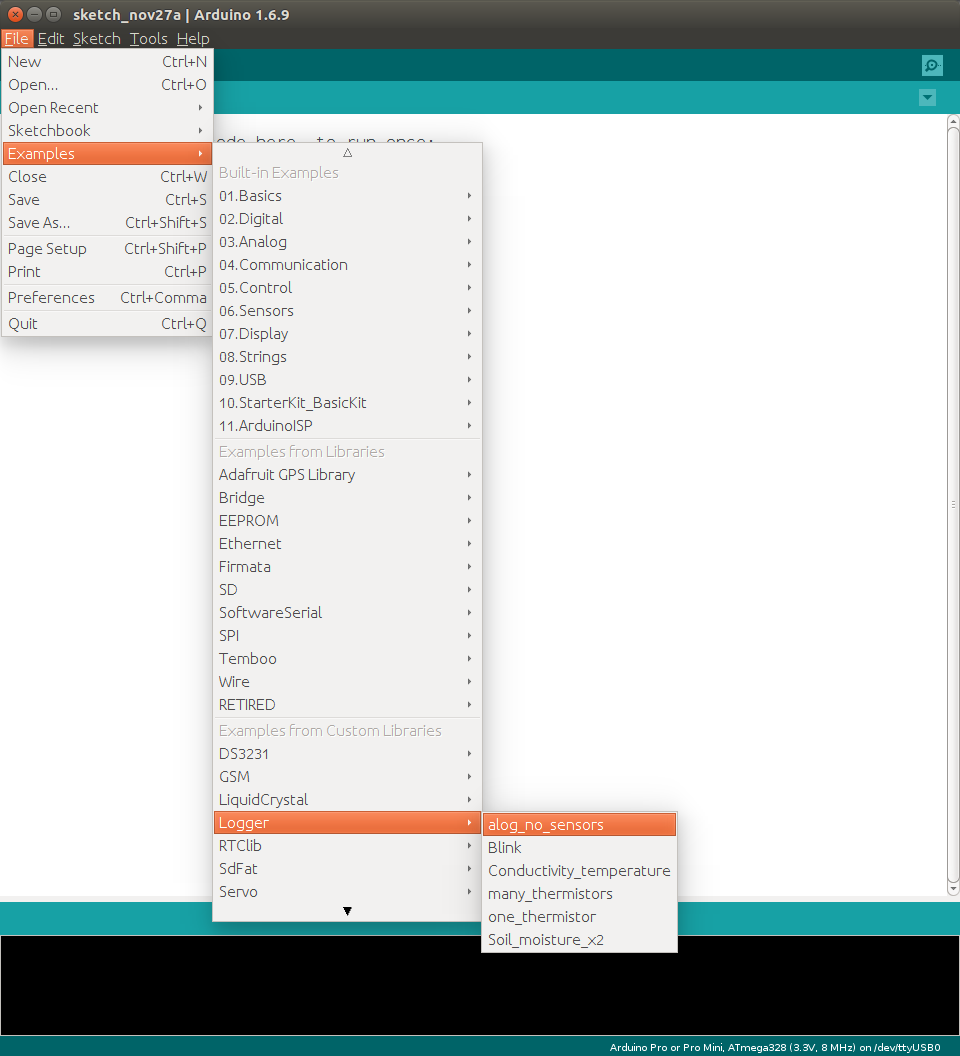
\includegraphics[width=.8\linewidth]{Open_alog_no_sensors.png}
\caption{Open alog\+\_\+no\+\_\+sensors\+: this is our blank template upon which you can write your logger code. For now, we will just upload this file alone.}
\end{DoxyImage}

\item Select \char`\"{}\+Arduino Pro\char`\"{} under \char`\"{}boards\char`\"{}. Sparkfun’s Arduino Pro 3.\+3V has the same microcontroller chip and clock speed as the A\+Log Bottle\+Logger, so its settings are compatible.  
\begin{DoxyImage}
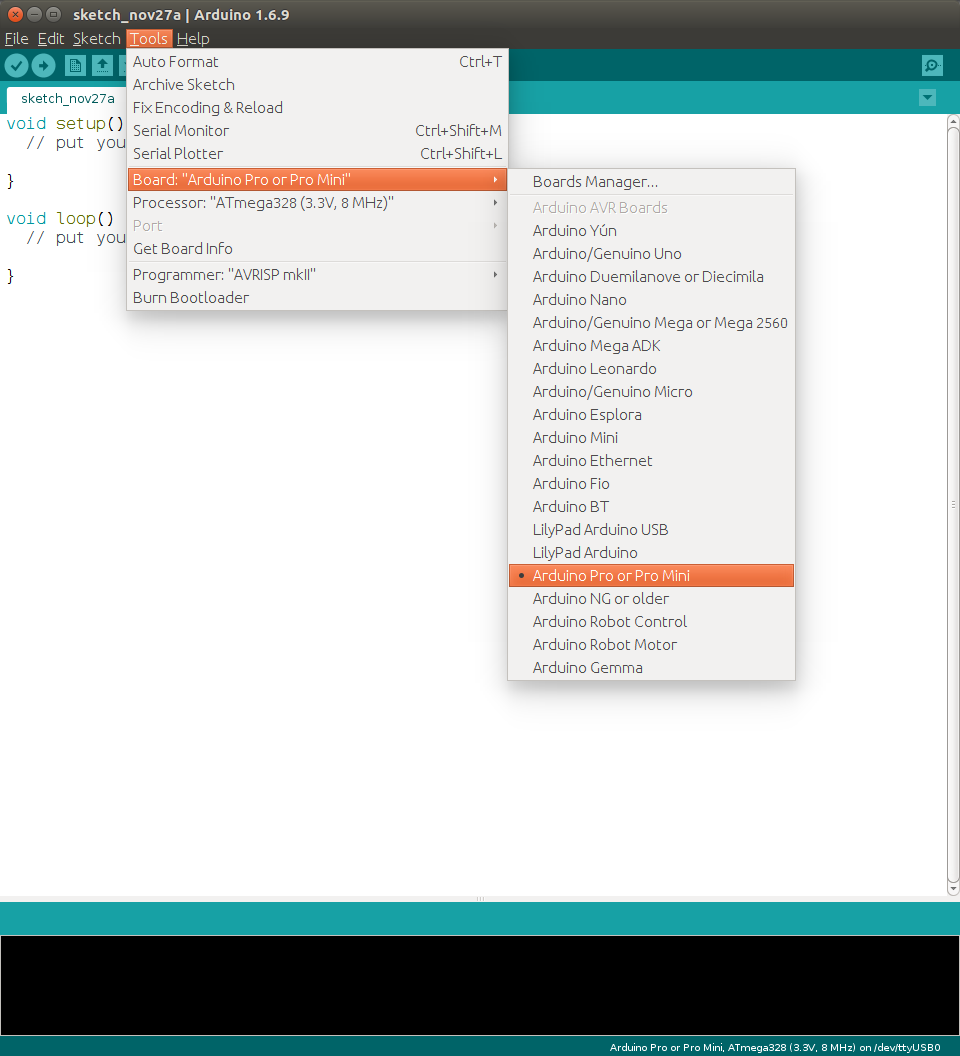
\includegraphics[width=.8\linewidth]{BoardsSelect_ArduinoPro.png}
\caption{Sparkfun\textquotesingle{}s Arduino pro can have the same settings as the A\+Log.}
\end{DoxyImage}

\item Select the processor for the A\+Log\+: 8 M\+Hz Arduino Pro 328.  
\begin{DoxyImage}
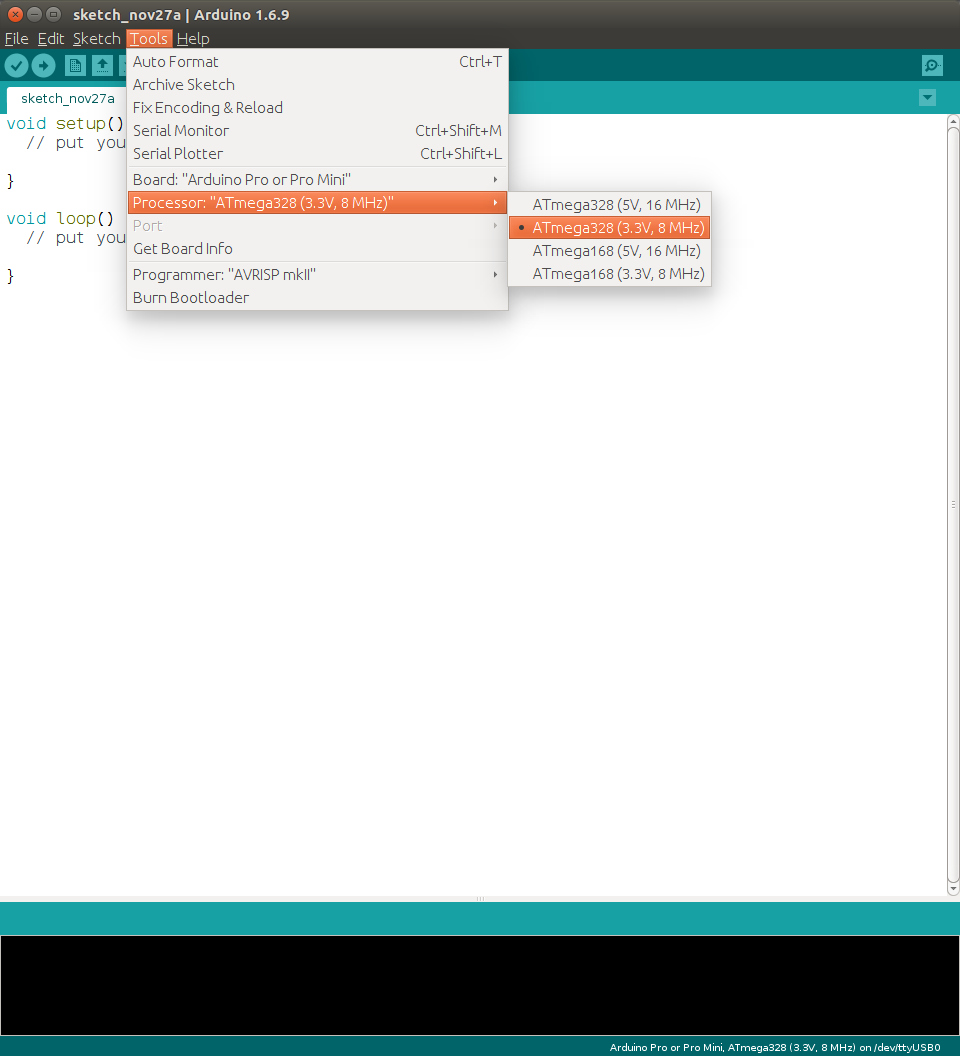
\includegraphics[width=.8\linewidth]{ProcessorSelect_3V3_8MHz.png}
\caption{The Arduino Pro or Pro Mini (3.3V, 8 M\+Hz) w/ A\+Tmega328 has the proper settings for the A\+Log Bottle\+Logger. Your version of Arduino won’t have the \textquotesingle{}A\+Log Bottle\+Logger\textquotesingle{} custom setting at the top; it is part of our work to eventually have a more streamlined A\+Log programming interface.}
\end{DoxyImage}

\item Plug in your A\+Log Bottle\+Logger using a U\+SB A to B cable.
\item The Bottle\+Logger should blink a couple of times on the L\+E\+D’s that are right by the U\+SB port. This means that it sees that it has been plugged in. Sometimes, we ship the Bottle\+Loggers with a \char`\"{}blink\char`\"{} program installed. This will cause the large red L\+ED in the center to blink when the A\+Log is plugged in... so your board might do this too. It’s one of our ways of testing that the board is programmable before shipping it to you.
\item Click on the \char`\"{}tools\char`\"{} menu, like the above figure. The \char`\"{}\+Serial Port\char`\"{} item in that menu should no longer be grayed out. Select your serial port.
\item Click \char`\"{}upload\char`\"{} from within the window holding \char`\"{}alog\+\_\+no\+\_\+sensors\char`\"{}, and send the code to the A\+Log. It will compile for a little while first, and then be sent over as a bitstream while the two small L\+E\+D’s by the U\+SB port on the A\+Log blink furiously\+: these are telling you that data is being sent to the logger (RX) or transmitted from the logger to the computer (TX).
\item Once this is done, click the \char`\"{}\+Serial Monitor\char`\"{} button to see what your data logger says. It will probably say something about setting the clock while the A\+Log flashes a syncopated rhythm on its main L\+ED. This means that it is time for your next step...
\end{DoxyEnumerate}\hypertarget{index_clock_setting}{}\subsection{Interfacing with the A\+Log and setting its clock}\label{index_clock_setting}
To set the clock of the A\+Log, plug it into your computer and run the \char`\"{}\+A\+Log\+Talk.\+py\char`\"{} program. This requires a Python interpreter (standard on all Linux and Mac computers) and can be done from the terminal by navigating to the A\+Log\+Talk directory and doing one of two things.

First, if you have a standard

F\+I\+N\+I\+SH T\+H\+IS A\+F\+T\+ER W\+O\+R\+K\+I\+NG T\+H\+R\+O\+U\+GH C\+L\+O\+CK S\+E\+T\+T\+I\+NG P\+R\+O\+G\+R\+A\+M\+S! S\+EE IF Y\+OU C\+AN G\+ET T\+HE H\+A\+N\+D\+S\+H\+A\+KE TO W\+O\+R\+K!

\begin{quote}
\begin{quote}
\begin{quote}
python A\+Log\+Talk.\+py \end{quote}
\end{quote}
\end{quote}


Instructions will appear on the screen; if the logger does not respond, you can push its \char`\"{}reset\char`\"{} button.

\begin{quote}
\begin{quote}
\begin{quote}
python A\+Log\+Talk.\+py \end{quote}
\end{quote}
\end{quote}


Instructions will appear on the screen; if the logger does not respond, you can push its \char`\"{}reset\char`\"{} button.\hypertarget{index_programming_your_own}{}\subsection{Creating and uploading a custom data logging routine}\label{index_programming_your_own}
The Github repository has examples of data logging routines, which you can modify for your own purposes. See the \char`\"{}examples\char`\"{} folder. You can also look at \char`\"{}\+Logger.\+h\char`\"{} to see what variables you need to pass to each sensor’s function.

These examples include comments for where you should place your commands to communicate with various sensors, both analog and digital.

If you are unfamiliar with C or Arduino programming, the Arduino reference guide can help\+: \href{http://arduino.cc/en/Reference/HomePage}{\tt http\+://arduino.\+cc/en/\+Reference/\+Home\+Page}.

{\bfseries I\+M\+P\+O\+R\+T\+A\+NT\+:} many examples of A\+Log code are included in this package; please use them as possible starting points for your code.\hypertarget{index_attaching_sensors}{}\subsection{Attaching sensors}\label{index_attaching_sensors}
Use the screw terminals (labeled) to connect sensors to the logger. These screw terminals are labeled with pin numbers that correspond to the pin numbers used in the program.\hypertarget{index_self_made_sensor_code}{}\subsection{Writing your own sensor code}\label{index_self_made_sensor_code}
\hypertarget{index_field_deployment}{}\subsection{Field deployment}\label{index_field_deployment}
We have learned a bit from past field installations, so you can e-\/mail us at \href{mailto:info@northernwidget.com}{\tt info@northernwidget.\+com} to tell us that you want some of these examples on the website. In the meantime, it’s basically an exercise in keeping the logger away from the elements and animals that like to chew wires.\hypertarget{index_pinout}{}\section{A\+Log pinout and peripherals}\label{index_pinout}
 
\begin{DoxyImage}
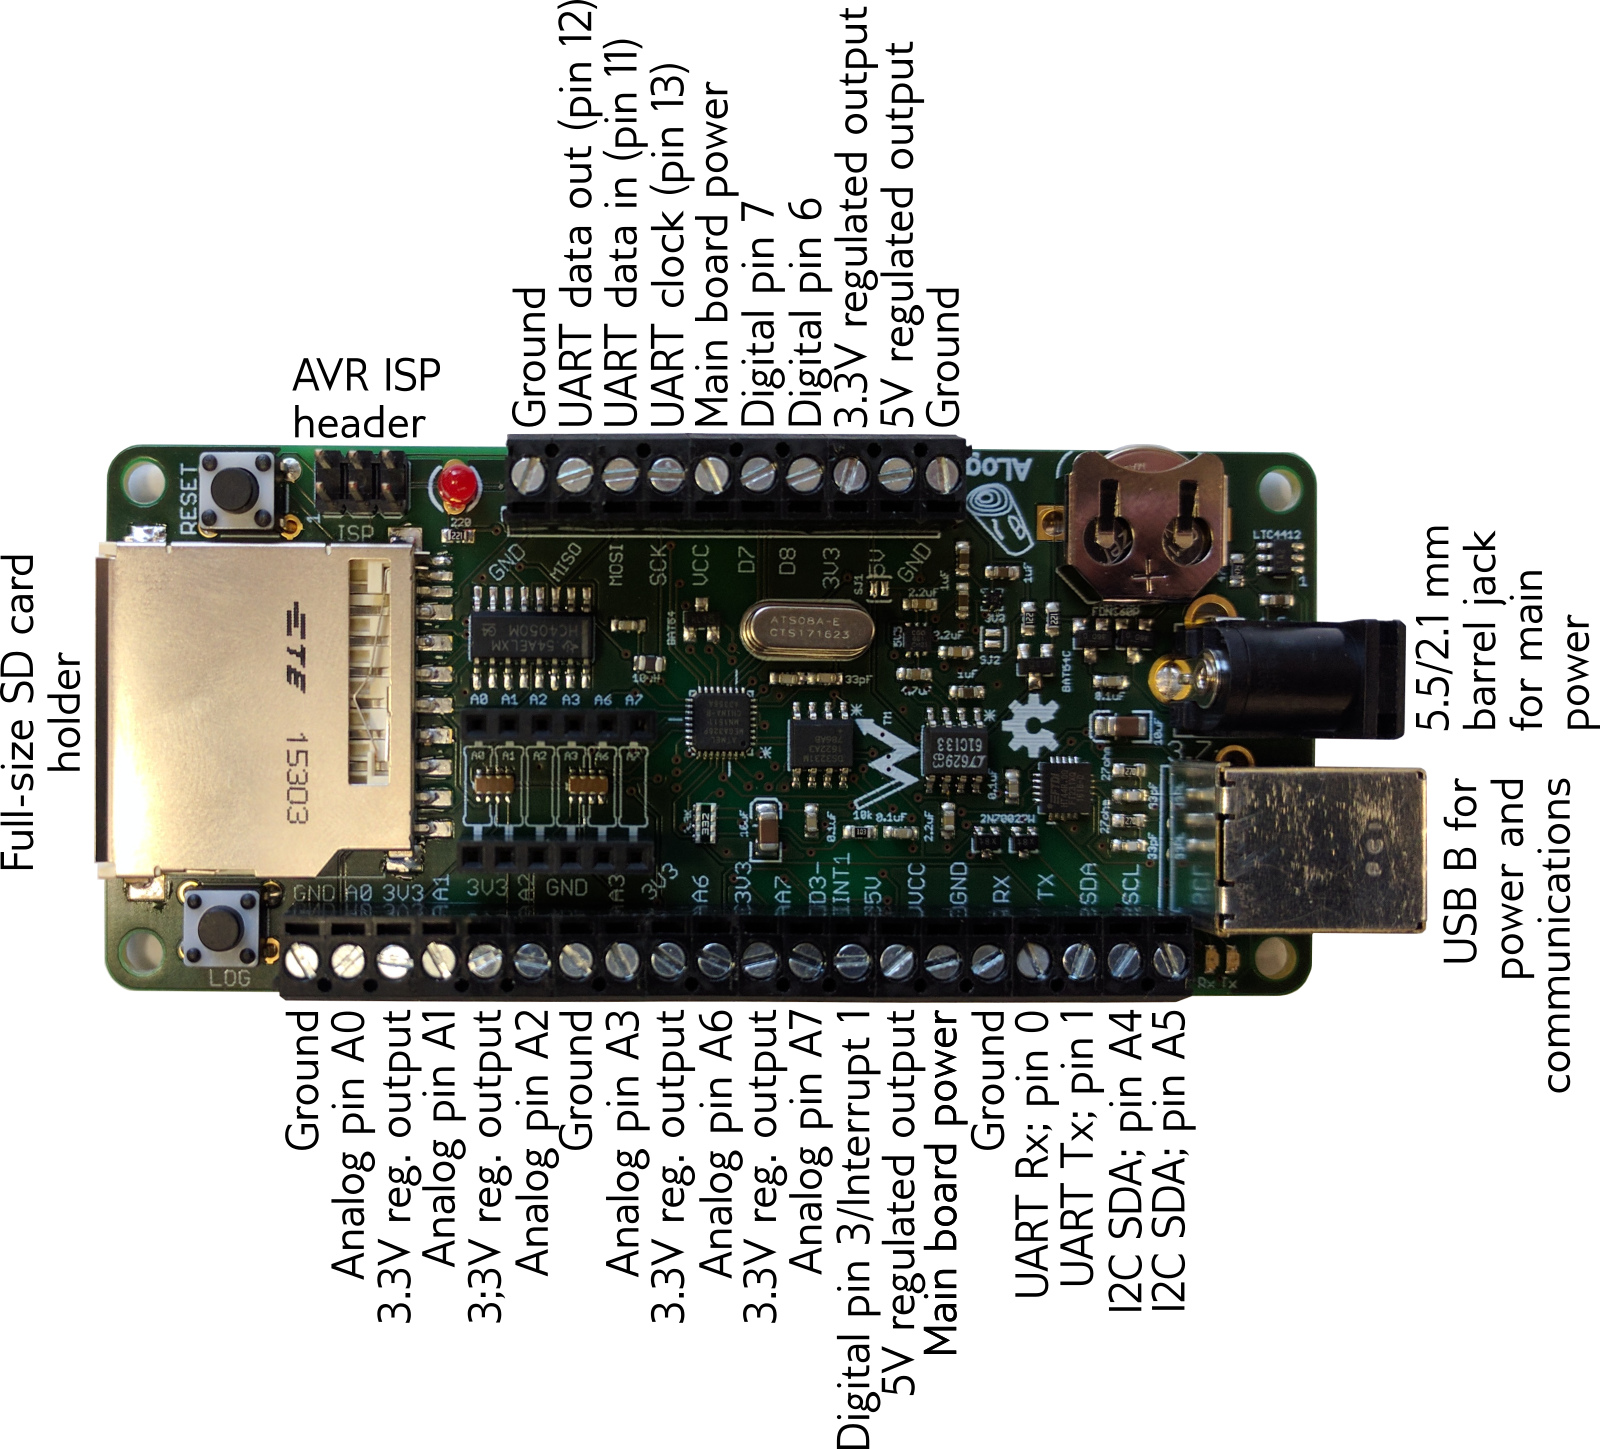
\includegraphics[width=\linewidth]{LoggerPinout.png}
\caption{A\+Log pinout and peripherals.}
\end{DoxyImage}


{\bfseries Notes} 
\begin{DoxyEnumerate}
\item All pin numbers correspond to those of the Arduino Uno
\item All S\+PI pins (11, 12, 13) are also used for SD card communication)
\item V\+CC means \char`\"{}\+Voltage of the Common Connector\char`\"{}
\item The 3.\+3V regulator is typically a precision voltage reference (part number L\+T1461\+D\+H\+S8-\/5\#\+P\+BF) that can source 10-\/50 mA of power, depending on V\+CC\+: 10 mA corresponds to 0.\+20V dropout between V\+CC and 3.\+3V; 50 mA corresponds to 1.\+5V dropout. Projects that need more power and/or use fully ratiometric measurements can request an A\+Log without this part; solder jumpers on the board will connect 3\+V3 pins to the unused side of our standard 3.\+3V low-\/dropout regulator.
\item The 5V regulated output is supplied via a charge pump; when no current is drawn, its voltage will increase to 5.\+2V; after some current draw, is output will drop to a stable 5V. If there is a concern about low voltage draw from the charge pump, users should monitor its voltage with a voltage divider connected to one of the analog channels, and include a reading during the time that the sensor or other load on the charge pump is on and active.
\item The interrupt pin (digital pin 3) can be used to detect events, such as an anemometer spinning or a rain gauge bucket tipping.
\end{DoxyEnumerate}\hypertarget{index_About}{}\section{About}\label{index_About}
Who is Northern Widget? What is the connection to the University of Minnesota?

{\bfseries Northern Widget} is a company that 
\chapter{Logger}
\label{md_README}
\Hypertarget{md_README}
\char`\"{}\+Logger\char`\"{} is the data logger library for the Arduino-\/based A\+Log (\href{http://northernwidget.com/alog/}{\tt http\+://northernwidget.\+com/alog/}) developed by Andy Wickert and Chad Sandell at Northern Widget L\+LC and the University of Minnesota.

While it is developed to work specifically with the A\+Log, it will also work with a standard Arduino that is outfitted with a SD card and a D\+S3231 real-\/time clock.

\char`\"{}\+Logger\char`\"{} is optimized to handle all of the basic file, system, and power management behind-\/the-\/scenes, and to reduce power consumption to minimal levels through the use of the sleep functions. It exposes sensor functions as single-\/line calls, and includes a template for the addition of new sensors.

For questions related to the \hyperlink{classLogger}{Logger} library, please send a message to us at \href{mailto:info@northernwidget.com}{\tt info@northernwidget.\+com}. 
\chapter{Class Index}
\section{Class List}
Here are the classes, structs, unions and interfaces with brief descriptions\+:\begin{DoxyCompactList}
\item\contentsline{section}{\hyperlink{classLogger}{Logger} }{\pageref{classLogger}}{}
\end{DoxyCompactList}

\chapter{File Index}
\section{File List}
Here is a list of all documented files with brief descriptions\+:\begin{DoxyCompactList}
\item\contentsline{section}{\hyperlink{Logger_8cpp}{Logger.\+cpp} }{\pageref{Logger_8cpp}}{}
\item\contentsline{section}{\hyperlink{Logger_8h}{Logger.\+h} }{\pageref{Logger_8h}}{}
\end{DoxyCompactList}

\chapter{Class Documentation}
\hypertarget{classLogger}{}\section{Logger Class Reference}
\label{classLogger}\index{Logger@{Logger}}
\subsection*{Public Member Functions}
\begin{DoxyCompactItemize}
\item 
\hyperlink{classLogger_abc41bfb031d896170c7675fa96a6b30c}{Logger} ()
\begin{DoxyCompactList}\small\item\em \hyperlink{classLogger}{Logger} library for the Arduino-\/based A\+Log data logger. \end{DoxyCompactList}\item 
void \hyperlink{classLogger_a635c5dc0046646bec7023ef7133f0eb3}{initialize} (char $\ast$\+\_\+logger\+\_\+name, char $\ast$\+\_\+datafilename, int \+\_\+hour\+Interval, int \+\_\+min\+Interval, int \+\_\+sec\+Interval, bool \+\_\+ext\+\_\+int=false, bool \+\_\+\+L\+O\+G\+\_\+\+O\+N\+\_\+\+B\+U\+C\+K\+E\+T\+\_\+\+T\+IP=false)
\item 
void \hyperlink{classLogger_ab5e0bd543758c65a17b77553a0e9f0c9}{setup\+Logger} ()
\item 
void \hyperlink{classLogger_ad90ff8f29410f6b70cc6334391400a4e}{sleep} ()
\item 
void \hyperlink{classLogger_ad28cf6450ada04f0e1475998bede5b88}{go\+To\+Sleep\+\_\+if\+\_\+needed} ()
\item 
void \hyperlink{classLogger_a4a6c78dd1715b33ae4bbd6f66f116f77}{start\+Logging} ()
\item 
void \hyperlink{classLogger_aa82814d61687debcf3b8dd6f46c9d549}{end\+Logging} ()
\item 
void \hyperlink{classLogger_af936c7f58e23316abb5614cbd31c7ced}{start\+Analog} ()
\item 
void \hyperlink{classLogger_adca7be8a63592263c67f63766680d16f}{end\+Analog} ()
\item 
bool \hyperlink{classLogger_acc758b6fdaac8099c492929aa7f1691d}{get\+\_\+use\+\_\+sleep\+\_\+mode} ()
\item 
float \hyperlink{classLogger_a343fcabefb37e06429865a2e6a6e708a}{read\+Pin} (int pin)
\item 
float \hyperlink{classLogger_a4e67526c65fa865f276a515a200af4aa}{read\+Pin\+Oversample} (int pin, int bits)
\item 
float \hyperlink{classLogger_ad8296890a14a0df83c2433a20f25b899}{analog\+Read\+Oversample} (int pin, uint8\+\_\+t adc\+\_\+bits=10, int nsamples=1, bool debug=false)
\item 
float \hyperlink{classLogger_a55d923b98a6c503fccb25bfd4af32f3d}{thermistorB} (float R0, float B, float Rref, float T0degC, int therm\+Pin, uint8\+\_\+t A\+D\+C\+\_\+resolution\+\_\+nbits=14, bool Rref\+\_\+on\+\_\+\+G\+N\+D\+\_\+side=true, bool oversample\+\_\+debug=false, bool record\+\_\+results=true)
\item 
void \hyperlink{classLogger_a362a1462166d63ddc613eaa1e86f9854}{ultrasonic\+M\+B\+\_\+analog\+\_\+1cm} (int nping, int EX, int sonic\+Pin, bool write\+All)
\item 
float \hyperlink{classLogger_a87ce56cb9c3dfc7abfd6308b2ee7dc10}{maxbotix\+H\+R\+X\+L\+\_\+\+W\+R\+\_\+\+Serial} (int Ex, int nping, bool write\+All, int max\+Range, bool R\+S232=false)
\item 
void \hyperlink{classLogger_a3ce2869bbd48fdebbf44e155981c85b0}{maxbotix\+H\+R\+X\+L\+\_\+\+W\+R\+\_\+analog} (int nping=10, int sonic\+Pin=A0, int EX=99, bool write\+All=true, uint8\+\_\+t A\+D\+C\+\_\+resolution\+\_\+nbits=10)
\item 
void \hyperlink{classLogger_a40ae372dee7f672a6d6f33ab441e4da1}{Decagon5\+TE} (int excit\+Pin, int data\+Pin)
\item 
void \hyperlink{classLogger_a84da6a9ec3d4d56fdc32d950b71f1a26}{Decagon\+G\+S1} (int pin, float Vref, uint8\+\_\+t A\+D\+C\+\_\+resolution\+\_\+nbits=14)
\item 
void \hyperlink{classLogger_ab1ae31b2bdb77c86fb6851907258171b}{vdivR} (int pin, float Rref, uint8\+\_\+t A\+D\+C\+\_\+resolution\+\_\+nbits=10, bool Rref\+\_\+on\+\_\+\+G\+N\+D\+\_\+side=true)
\item 
void \hyperlink{classLogger_a95670d06ec3b68300895cd7bf8c37999}{linear\+Potentiometer} (int linpot\+Pin, float Rref, float slope, char $\ast$\+\_\+distance\+\_\+units, float intercept=0, uint8\+\_\+t A\+D\+C\+\_\+resolution\+\_\+nbits=14, bool Rref\+\_\+on\+\_\+\+G\+N\+D\+\_\+side=true)
\item 
void \hyperlink{classLogger_a4ccff7a14a6bddc8bb28e22b3b36d3cc}{H\+T\+M2500\+L\+F\+\_\+humidity\+\_\+temperature} (int humid\+Pin, int therm\+Pin, float Rref\+\_\+therm, uint8\+\_\+t A\+D\+C\+\_\+resolution\+\_\+nbits=14)
\item 
void \hyperlink{classLogger_a62b74ddb3cf9fdd7dae2394c1b245ed4}{H\+M1500\+L\+F\+\_\+humidity\+\_\+with\+\_\+external\+\_\+temperature} (int humid\+Pin, float R0\+\_\+therm, float B\+\_\+therm, float Rref\+\_\+therm, float T0deg\+C\+\_\+therm, int therm\+Pin\+\_\+therm, uint8\+\_\+t A\+D\+C\+\_\+resolution\+\_\+nbits=14)
\item 
void \hyperlink{classLogger_a80fdea5a339573980f9544ac64678411}{Inclinometer\+\_\+\+S\+C\+A100\+T\+\_\+\+D02\+\_\+analog\+\_\+\+Tcorr} (int x\+Pin, int y\+Pin, float Vref, float Vsupply, float R0\+\_\+therm, float B\+\_\+therm, float Rref\+\_\+therm, float T0deg\+C\+\_\+therm, int therm\+Pin\+\_\+therm, uint8\+\_\+t A\+D\+C\+\_\+resolution\+\_\+nbits=14)
\item 
void \hyperlink{classLogger_a6c6a43a1b86f88c2a5e33d14c992e510}{Anemometer\+\_\+reed\+\_\+switch} (int interrupt\+\_\+pin\+\_\+number, unsigned long reading\+\_\+duration\+\_\+milliseconds, float meters\+\_\+per\+\_\+second\+\_\+per\+\_\+rotation)
\item 
void \hyperlink{classLogger_a31c3cba5ff5722fb66bf540bfbe8b25d}{Wind\+\_\+\+Vane\+\_\+\+Inspeed} (int vane\+Pin)
\item 
void \hyperlink{classLogger_ae4190ce7ccfd7b148a6151102a3bf93d}{Pyranometer} (int analog\+Pin, float raw\+\_\+m\+V\+\_\+per\+\_\+\+W\+\_\+per\+\_\+m2, float gain, float V\+\_\+ref, uint8\+\_\+t A\+D\+C\+\_\+resolution\+\_\+nbits=14)
\item 
void \hyperlink{classLogger_a40588117a274f0c6de926ef6ce1f0ba8}{Barometer\+\_\+\+B\+M\+P180} ()
\item 
void \hyperlink{classLogger_a98f3cc370c87d1e1eaf3eb6a7e0f1623}{\+\_\+sensor\+\_\+function\+\_\+template} (int pin, float param1, float param2, int A\+D\+C\+\_\+bits=14, bool flag=false)
\item 
void \hyperlink{classLogger_a923b296832bd4222da649ebc66427ac1}{Hack\+HD} (int control\+\_\+pin, bool want\+\_\+camera\+\_\+on)
\item 
float \hyperlink{classLogger_a9808967fdf91f10602aa883df35145b3}{Honeywell\+\_\+\+H\+S\+C\+\_\+analog} (int pin, float Vsupply, float Vref, float Pmin, float Pmax, int Transfer\+Function\+\_\+number, int units, uint8\+\_\+t A\+D\+C\+\_\+resolution\+\_\+nbits=14)
\end{DoxyCompactItemize}


\subsection{Constructor \& Destructor Documentation}
\mbox{\Hypertarget{classLogger_abc41bfb031d896170c7675fa96a6b30c}\label{classLogger_abc41bfb031d896170c7675fa96a6b30c}} 
\index{Logger@{Logger}!Logger@{Logger}}
\index{Logger@{Logger}!Logger@{Logger}}
\subsubsection{\texorpdfstring{Logger()}{Logger()}}
{\footnotesize\ttfamily Logger\+::\+Logger (\begin{DoxyParamCaption}{ }\end{DoxyParamCaption})}



\hyperlink{classLogger}{Logger} library for the Arduino-\/based A\+Log data logger. 

A\+Log data logger library\+: methods to\+:
\begin{DoxyItemize}
\item Initialize the data logger
\item Sleep and wake
\item Interact with the real-\/time clock (R\+TC)
\item Write data to the SD card
\item Manage power
\item Interact with a range of sensors
\end{DoxyItemize}

All help documentation here assumes you have created an instance of the \char`\"{}\+Logger\char`\"{} 
\begin{DoxyCode}
logger \hyperlink{classLogger_abc41bfb031d896170c7675fa96a6b30c}{Logger}();
\end{DoxyCode}
 

\subsection{Member Function Documentation}
\mbox{\Hypertarget{classLogger_a98f3cc370c87d1e1eaf3eb6a7e0f1623}\label{classLogger_a98f3cc370c87d1e1eaf3eb6a7e0f1623}} 
\index{Logger@{Logger}!\+\_\+sensor\+\_\+function\+\_\+template@{\+\_\+sensor\+\_\+function\+\_\+template}}
\index{\+\_\+sensor\+\_\+function\+\_\+template@{\+\_\+sensor\+\_\+function\+\_\+template}!Logger@{Logger}}
\subsubsection{\texorpdfstring{\+\_\+sensor\+\_\+function\+\_\+template()}{\_sensor\_function\_template()}}
{\footnotesize\ttfamily void Logger\+::\+\_\+sensor\+\_\+function\+\_\+template (\begin{DoxyParamCaption}\item[{int}]{pin,  }\item[{float}]{param1,  }\item[{float}]{param2,  }\item[{int}]{A\+D\+C\+\_\+bits = {\ttfamily 14},  }\item[{bool}]{flag = {\ttfamily false} }\end{DoxyParamCaption})}

Function to help lay out a new sensor interface. This need not be \char`\"{}void\char`\"{}\+: it may return a value as well.

Details about sensor go here


\begin{DoxyParams}{Parameters}
{\em pin} & You often need to specify interface pins\\
\hline
{\em param1} & A variable for the sensor or to interpret its value\\
\hline
{\em param2} & A variable for the sensor or to interpret its value\\
\hline
{\em A\+D\+C\+\_\+bits} & You often need to specify how much the analog-\/to-\/digital converter should be oversampled; this can range from 10 (no oversampling) to 16 (maximum possible oversampling before certainty in the oversampling method drops)\\
\hline
{\em flag} & Something that helps to set an option\\
\hline
\end{DoxyParams}
Example (made up)\+: 
\begin{DoxyCode}
logger.Example(A2, 1021.3, 15.2, True);
\end{DoxyCode}
\mbox{\Hypertarget{classLogger_ad8296890a14a0df83c2433a20f25b899}\label{classLogger_ad8296890a14a0df83c2433a20f25b899}} 
\index{Logger@{Logger}!analog\+Read\+Oversample@{analog\+Read\+Oversample}}
\index{analog\+Read\+Oversample@{analog\+Read\+Oversample}!Logger@{Logger}}
\subsubsection{\texorpdfstring{analog\+Read\+Oversample()}{analogReadOversample()}}
{\footnotesize\ttfamily float Logger\+::analog\+Read\+Oversample (\begin{DoxyParamCaption}\item[{int}]{pin,  }\item[{uint8\+\_\+t}]{adc\+\_\+bits = {\ttfamily 10},  }\item[{int}]{nsamples = {\ttfamily 1},  }\item[{bool}]{debug = {\ttfamily false} }\end{DoxyParamCaption})}

Higher analog resolution through oversampling

This function incorporates oversampling to extend the A\+DC precision past ten bits by taking more readings and statistically combing them.

Returns a floating point number between 0 and 1023 in order to be intechangable with the Arduino core Analog\+Read() function

It is often used within other sensor functinons to increase measurement precision.


\begin{DoxyParams}{Parameters}
{\em pin} & is the analog pin number\\
\hline
{\em adc\+\_\+bits} & is the reading precision in bits (2$^\wedge$adc\+\_\+bits). The A\+T\+Mega328 (Arduino Uno and A\+Log Bottle\+Logger core chip) has a base A\+DC precision of 10 bits (returns values of 0-\/1023) A reasonable maximum precision gain is (base\+\_\+value\+\_\+bits)+6, so 16 bits is a reasonable maximum precision for the A\+Log Bottle\+Logger.\\
\hline
{\em nsamples} & is the number of times you want to poll the particular sensor and write the output to file.\\
\hline
{\em debug} & is a flag that, if true, will write all of the values read during the oversampling to \char`\"{}\+Oversample.\+txt\char`\"{}.\\
\hline
\end{DoxyParams}
Example\+: 
\begin{DoxyCode}
\textcolor{comment}{// 12-bit measurement of Pin 2}
\textcolor{comment}{// Leaves nsamples at its default value of 1 (single reading of sensor)}
logger.analogReadOversample(2, 12);
\end{DoxyCode}


Readings that require more bits of precision will take longer.

For analog measurements that do not require more than 10 bits of precision, use logger.\+readpin(int pin) or the standard Arduino \char`\"{}\+Analog\+Read\char`\"{} function.

Based on e\+R\+Ca\+Guy\+\_\+\+New\+Analog\+Read\+::take\+Samples(uint8\+\_\+t analog\+Pin)

Example\+: 
\begin{DoxyCode}
\textcolor{comment}{// Take a single sample at 14-bit resolution and store it as "myReading"}
myReading = logger.analogReadOversample(A3, 14, 1);
\end{DoxyCode}
\mbox{\Hypertarget{classLogger_a6c6a43a1b86f88c2a5e33d14c992e510}\label{classLogger_a6c6a43a1b86f88c2a5e33d14c992e510}} 
\index{Logger@{Logger}!Anemometer\+\_\+reed\+\_\+switch@{Anemometer\+\_\+reed\+\_\+switch}}
\index{Anemometer\+\_\+reed\+\_\+switch@{Anemometer\+\_\+reed\+\_\+switch}!Logger@{Logger}}
\subsubsection{\texorpdfstring{Anemometer\+\_\+reed\+\_\+switch()}{Anemometer\_reed\_switch()}}
{\footnotesize\ttfamily void Logger\+::\+Anemometer\+\_\+reed\+\_\+switch (\begin{DoxyParamCaption}\item[{int}]{interrupt\+\_\+pin\+\_\+number,  }\item[{unsigned long}]{reading\+\_\+duration\+\_\+milliseconds,  }\item[{float}]{meters\+\_\+per\+\_\+second\+\_\+per\+\_\+rotation }\end{DoxyParamCaption})}

Anemometer that flips a reed switch each time it spins.


\begin{DoxyParams}{Parameters}
{\em interrupt\+\_\+pin\+\_\+number} & is the digital pin number corresponding to the appropriate interrupt; it uses the Arduino digital\+Pin\+To\+Interrupt(n\+\_\+pin) function to properly attach the interrupt. On the A\+Log Bottle\+Logger, this number will always be {\bfseries 3}.\\
\hline
{\em reading\+\_\+duration\+\_\+milliseconds} & How long will you count revolutions? Shorter durations save power, longer durations increase accuracy; very long durations will produce long-\/term averages. Typical values are a few seconds.\\
\hline
{\em meters\+\_\+per\+\_\+second\+\_\+per\+\_\+rotation} & Conversion factor between revolutions and wind speed. For the Inspeed Vortex wind sensor that we have used (\href{http://www.inspeed.com/anemometers/Vortex_Wind_Sensor.asp}{\tt http\+://www.\+inspeed.\+com/anemometers/\+Vortex\+\_\+\+Wind\+\_\+\+Sensor.\+asp}), this is\+: {\bfseries 2.\+5 mph/\+Hz = 1.\+1176 (m/s)/\+Hz}\\
\hline
\end{DoxyParams}
This function depends on the global variable {\bfseries rotation\+\_\+count}.

Example\+: 
\begin{DoxyCode}
\textcolor{comment}{// 4-second reading with Inspeed Vortex wind sensor on digital pin 3}
\textcolor{comment}{// (interrupt 1), returned in meters per second}
logger.Anemometer\_reed\_switch(3, 4000, 1.1176);
\end{DoxyCode}
\mbox{\Hypertarget{classLogger_a40588117a274f0c6de926ef6ce1f0ba8}\label{classLogger_a40588117a274f0c6de926ef6ce1f0ba8}} 
\index{Logger@{Logger}!Barometer\+\_\+\+B\+M\+P180@{Barometer\+\_\+\+B\+M\+P180}}
\index{Barometer\+\_\+\+B\+M\+P180@{Barometer\+\_\+\+B\+M\+P180}!Logger@{Logger}}
\subsubsection{\texorpdfstring{Barometer\+\_\+\+B\+M\+P180()}{Barometer\_BMP180()}}
{\footnotesize\ttfamily void Logger\+::\+Barometer\+\_\+\+B\+M\+P180 (\begin{DoxyParamCaption}{ }\end{DoxyParamCaption})}

Read absolute pressure in mbar.

This function reads the absolute pressure in mbar (h\+Pa). B\+M\+P180 sensor incorporates on board temperature correction. Uses I2C protocol.

Example\+: 
\begin{DoxyCode}
logger.Barometer\_BMP180();
\end{DoxyCode}
\mbox{\Hypertarget{classLogger_a40ae372dee7f672a6d6f33ab441e4da1}\label{classLogger_a40ae372dee7f672a6d6f33ab441e4da1}} 
\index{Logger@{Logger}!Decagon5\+TE@{Decagon5\+TE}}
\index{Decagon5\+TE@{Decagon5\+TE}!Logger@{Logger}}
\subsubsection{\texorpdfstring{Decagon5\+T\+E()}{Decagon5TE()}}
{\footnotesize\ttfamily void Logger\+::\+Decagon5\+TE (\begin{DoxyParamCaption}\item[{int}]{excit\+Pin,  }\item[{int}]{data\+Pin }\end{DoxyParamCaption})}

Reads a Decagon Devices 5\+TE soil moisture probe.

N\+E\+E\+DS T\+E\+S\+T\+I\+NG with current A\+Log version.

Returns Dielectric permittivity \mbox{[}-\/unitless-\/\mbox{]}, electrical conductivity \mbox{[}d\+S/m\mbox{]}, and temperature \mbox{[}degrees C\mbox{]}. Soil moisture is calculated through postprocessing.

Uses {\bfseries Software\+Serial}, and therefore has the potential to go unstable; however, we have a time limit, so this won\textquotesingle{}t crash the logger\+: it will just keep the logger from recording good data.

Modified from Steve Hicks\textquotesingle{} code for an L\+CD reader by Andy Wickert


\begin{DoxyParams}{Parameters}
{\em excit\+Pin} & activates the probe and powers it\\
\hline
{\em data\+Pin} & receives incoming serial data at 1200 bps\\
\hline
\end{DoxyParams}
Example\+: 
\begin{DoxyCode}
logger.Decagon5TE(7, 8);
\end{DoxyCode}
\mbox{\Hypertarget{classLogger_a84da6a9ec3d4d56fdc32d950b71f1a26}\label{classLogger_a84da6a9ec3d4d56fdc32d950b71f1a26}} 
\index{Logger@{Logger}!Decagon\+G\+S1@{Decagon\+G\+S1}}
\index{Decagon\+G\+S1@{Decagon\+G\+S1}!Logger@{Logger}}
\subsubsection{\texorpdfstring{Decagon\+G\+S1()}{DecagonGS1()}}
{\footnotesize\ttfamily void Logger\+::\+Decagon\+G\+S1 (\begin{DoxyParamCaption}\item[{int}]{pin,  }\item[{float}]{Vref,  }\item[{uint8\+\_\+t}]{A\+D\+C\+\_\+resolution\+\_\+nbits = {\ttfamily 14} }\end{DoxyParamCaption})}

Ruggedized Decagon Devices soil moisture sensor


\begin{DoxyParams}{Parameters}
{\em pin} & Analog pin number\\
\hline
{\em Vref} & is the reference voltage of the A\+DC; on the A\+Log, this is a precision 3.\+3V regulator (unless a special unit without this regulator is ordered; the regulator uses significant power)\\
\hline
{\em A\+D\+C\+\_\+resolution\+\_\+nbits} & (10-\/16 for the A\+Log Bottle\+Logger) is the number of bits of A\+DC resolution used (oversampling for $>$10 bits)\\
\hline
\end{DoxyParams}
Example\+: 
\begin{DoxyCode}
\textcolor{comment}{// Using a non-precision Rref that is slightly off}
logger.DecagonGS1(A1, 3.27, 14);
\end{DoxyCode}
\mbox{\Hypertarget{classLogger_adca7be8a63592263c67f63766680d16f}\label{classLogger_adca7be8a63592263c67f63766680d16f}} 
\index{Logger@{Logger}!end\+Analog@{end\+Analog}}
\index{end\+Analog@{end\+Analog}!Logger@{Logger}}
\subsubsection{\texorpdfstring{end\+Analog()}{endAnalog()}}
{\footnotesize\ttfamily void Logger\+::end\+Analog (\begin{DoxyParamCaption}{ }\end{DoxyParamCaption})}

Turn off power to analog sensors\mbox{\Hypertarget{classLogger_aa82814d61687debcf3b8dd6f46c9d549}\label{classLogger_aa82814d61687debcf3b8dd6f46c9d549}} 
\index{Logger@{Logger}!end\+Logging@{end\+Logging}}
\index{end\+Logging@{end\+Logging}!Logger@{Logger}}
\subsubsection{\texorpdfstring{end\+Logging()}{endLogging()}}
{\footnotesize\ttfamily void Logger\+::end\+Logging (\begin{DoxyParamCaption}{ }\end{DoxyParamCaption})}

Endslogging and returns to sleep

Ends line, turns of SD card, and resets alarm\+: ready to sleep.

Also runs tipping bucket rain gauge code (function that records time stamp) if one is attached and activated.

{\bfseries I\+M\+P\+O\+R\+T\+A\+NT\+:} If the logger is not writing data to the card, and the card is properly inserted, the manually-\/set delay here may be the problem. We think we have made it long enough, but because it is hard-\/coded, there could be an unforeseen circumstance in which it is not!\mbox{\Hypertarget{classLogger_acc758b6fdaac8099c492929aa7f1691d}\label{classLogger_acc758b6fdaac8099c492929aa7f1691d}} 
\index{Logger@{Logger}!get\+\_\+use\+\_\+sleep\+\_\+mode@{get\+\_\+use\+\_\+sleep\+\_\+mode}}
\index{get\+\_\+use\+\_\+sleep\+\_\+mode@{get\+\_\+use\+\_\+sleep\+\_\+mode}!Logger@{Logger}}
\subsubsection{\texorpdfstring{get\+\_\+use\+\_\+sleep\+\_\+mode()}{get\_use\_sleep\_mode()}}
{\footnotesize\ttfamily bool Logger\+::get\+\_\+use\+\_\+sleep\+\_\+mode (\begin{DoxyParamCaption}{ }\end{DoxyParamCaption})}

Does the logger enter a low-\/power sleep mode? T/F.


\begin{DoxyItemize}
\item True if the logger is going to sleep between pases through the data-\/reading loop.
\item False if the logger is looping over its logging step (inside void loop() in the $\ast$.ino code) continuously without sleeping
\end{DoxyItemize}\mbox{\Hypertarget{classLogger_ad28cf6450ada04f0e1475998bede5b88}\label{classLogger_ad28cf6450ada04f0e1475998bede5b88}} 
\index{Logger@{Logger}!go\+To\+Sleep\+\_\+if\+\_\+needed@{go\+To\+Sleep\+\_\+if\+\_\+needed}}
\index{go\+To\+Sleep\+\_\+if\+\_\+needed@{go\+To\+Sleep\+\_\+if\+\_\+needed}!Logger@{Logger}}
\subsubsection{\texorpdfstring{go\+To\+Sleep\+\_\+if\+\_\+needed()}{goToSleep\_if\_needed()}}
{\footnotesize\ttfamily void Logger\+::go\+To\+Sleep\+\_\+if\+\_\+needed (\begin{DoxyParamCaption}{ }\end{DoxyParamCaption})}

Places logger into sleep mode iff this is being used.

Function is accessible from Arduino sketch; is designed for cases in which an external override may be required.\mbox{\Hypertarget{classLogger_a923b296832bd4222da649ebc66427ac1}\label{classLogger_a923b296832bd4222da649ebc66427ac1}} 
\index{Logger@{Logger}!Hack\+HD@{Hack\+HD}}
\index{Hack\+HD@{Hack\+HD}!Logger@{Logger}}
\subsubsection{\texorpdfstring{Hack\+H\+D()}{HackHD()}}
{\footnotesize\ttfamily void Logger\+::\+Hack\+HD (\begin{DoxyParamCaption}\item[{int}]{control\+\_\+pin,  }\item[{bool}]{want\+\_\+camera\+\_\+on }\end{DoxyParamCaption})}

Hack\+HD camera control function

Control the Hack\+HD camera\+: this function turns the Hack\+HD on or off and records the time stamp from when the Hack\+HD turns on/off in a file called \char`\"{}camera.\+txt\char`\"{}.

Because this function turns the camera on or off, you have to ensure that you write a mechanism to keep it on for some time in your code. This could be checking the time each time you wake and deciding what to do, for example. In short\+: this function is a lower-\/level utility that requires the end-\/user to write the rest of the camera control sequence themselves.


\begin{DoxyParams}{Parameters}
{\em control\+\_\+pin} & is the pin connected to the Hack\+HD on/off switch; Dropping control\+\_\+pin to G\+ND for 200 ms turns camera on or off.\\
\hline
{\em want\+\_\+camera\+\_\+on} & is true if you want to turn the camera on, false if you want to turn the camera off.\\
\hline
{\em C\+A\+M\+E\+R\+A\+\_\+\+I\+S\+\_\+\+ON} & is a global varaible attached to this function that saves the state of the camera; it will be compared to \char`\"{}want\+\_\+camera\+\_\+on\char`\"{}, such that this function will do nothing if the camera is already on (or off) and you want it on (or off).\\
\hline
\end{DoxyParams}
Power requirements\+:


\begin{DoxyItemize}
\item 0.\+2 mA quiescent current draw;
\item 600 mA while recording
\end{DoxyItemize}

Example (not tested)\+:


\begin{DoxyCode}
\textcolor{comment}{// Before "setup":}
uint32\_t t\_camera\_timeout\_start\_unixtime;
\textcolor{keywordtype}{int} timeout\_secs = 300;
book camera\_on = \textcolor{keyword}{false};
\textcolor{comment}{// ...}

\textcolor{comment}{// Inside "loop":}
\textcolor{comment}{// Turn the camera on after some triggering event, and keep it on for as }
\textcolor{comment}{// long as this condition is met, and for at least 5 minutes afterwards.}
\textcolor{comment}{// }
\textcolor{comment}{// >> some code to measure a variable's "distance"}
\textcolor{comment}{// ...}
\textcolor{comment}{// }
\textcolor{keywordflow}{if} (distance < 1500)\{
  logger.HackHD(8, \textcolor{keyword}{true});
  camera\_on = \textcolor{keyword}{true}; \textcolor{comment}{// Maybe I can get a global variable from this library}
                    \textcolor{comment}{// or have HackHD function return the camera state?}
  now = RTC.now();
  \textcolor{comment}{// Reset the timeout clock}
  t\_camera\_timeout\_start\_unixtime = now.unixtime(); 
\}
\textcolor{keywordflow}{else} \textcolor{keywordflow}{if}(camera\_on)\{
  now = RTC.now();
  \textcolor{comment}{// If timed out, turn it off.}
  \textcolor{keywordflow}{if} ((t\_camera\_timeout\_start\_unixtime - now.unixtime()) > timeout\_secs)\{
    logger.HackHD(8, \textcolor{keyword}{false});
    camera\_on = \textcolor{keyword}{false};
  \}
\}
\end{DoxyCode}


This example could be used to capture flow during a flash flood. See\+:
\begin{DoxyItemize}
\item Website\+: \href{http://instaar.colorado.edu/~wickert/atvis/}{\tt http\+://instaar.\+colorado.\+edu/$\sim$wickert/atvis/}
\item A\+GU poster\+: \href{https://www.researchgate.net/publication/241478936_The_Automatically_Triggered_Video_or_Imaging_Station_ATVIS_An_Inexpensive_Way_to_Catch_Geomorphic_Events_on_Camera}{\tt https\+://www.\+researchgate.\+net/publication/241478936\+\_\+\+The\+\_\+\+Automatically\+\_\+\+Triggered\+\_\+\+Video\+\_\+or\+\_\+\+Imaging\+\_\+\+Station\+\_\+\+A\+T\+V\+I\+S\+\_\+\+An\+\_\+\+Inexpensive\+\_\+\+Way\+\_\+to\+\_\+\+Catch\+\_\+\+Geomorphic\+\_\+\+Events\+\_\+on\+\_\+\+Camera}
\end{DoxyItemize}\mbox{\Hypertarget{classLogger_a62b74ddb3cf9fdd7dae2394c1b245ed4}\label{classLogger_a62b74ddb3cf9fdd7dae2394c1b245ed4}} 
\index{Logger@{Logger}!H\+M1500\+L\+F\+\_\+humidity\+\_\+with\+\_\+external\+\_\+temperature@{H\+M1500\+L\+F\+\_\+humidity\+\_\+with\+\_\+external\+\_\+temperature}}
\index{H\+M1500\+L\+F\+\_\+humidity\+\_\+with\+\_\+external\+\_\+temperature@{H\+M1500\+L\+F\+\_\+humidity\+\_\+with\+\_\+external\+\_\+temperature}!Logger@{Logger}}
\subsubsection{\texorpdfstring{H\+M1500\+L\+F\+\_\+humidity\+\_\+with\+\_\+external\+\_\+temperature()}{HM1500LF\_humidity\_with\_external\_temperature()}}
{\footnotesize\ttfamily void Logger\+::\+H\+M1500\+L\+F\+\_\+humidity\+\_\+with\+\_\+external\+\_\+temperature (\begin{DoxyParamCaption}\item[{int}]{humid\+Pin,  }\item[{float}]{R0\+\_\+therm,  }\item[{float}]{B\+\_\+therm,  }\item[{float}]{Rref\+\_\+therm,  }\item[{float}]{T0deg\+C\+\_\+therm,  }\item[{int}]{therm\+Pin\+\_\+therm,  }\item[{uint8\+\_\+t}]{A\+D\+C\+\_\+resolution\+\_\+nbits = {\ttfamily 14} }\end{DoxyParamCaption})}

H\+M1500\+LF Relative humidity sensor with external temperature correction

This function measures the relative humidity of using a H\+T\+M1500 relative humidity sensor and an external thermistor. The relative humidity and temperature are measured using an oversampling method. Results are displayed on the serial monitor and saved onto the SD card to four decimal places. Temperature and relative humidity are recorded.


\begin{DoxyParams}{Parameters}
{\em humid\+Pin} & is the analog pin connected to the humidity output voltage of the module.\\
\hline
{\em R0\+\_\+therm} & is the resistance of the thermistor at the known temperature.\\
\hline
{\em B\+\_\+therm} & is the B-\/ or β-\/ parameter of the thermistor.\\
\hline
{\em Rref\+\_\+therm} & is the resistance of the corresponding reference resistor for that analog pin.\\
\hline
{\em T0deg\+C\+\_\+therm} & is a thermistor calibration.\\
\hline
{\em therm\+Pin\+\_\+therm} & is the analog pin connected to the tempurature output voltage of the module.\\
\hline
{\em A\+D\+C\+\_\+resolution\+\_\+nbits} & (10-\/16 for the A\+Log Bottle\+Logger) is the number of bits of A\+DC resolution used (oversampling for $>$10)\\
\hline
\end{DoxyParams}
Example\+: 
\begin{DoxyCode}
logger.HM1500LF\_humidity\_with\_external\_temperature1,10000,3950,10000,25,1,12);
\end{DoxyCode}
\mbox{\Hypertarget{classLogger_a9808967fdf91f10602aa883df35145b3}\label{classLogger_a9808967fdf91f10602aa883df35145b3}} 
\index{Logger@{Logger}!Honeywell\+\_\+\+H\+S\+C\+\_\+analog@{Honeywell\+\_\+\+H\+S\+C\+\_\+analog}}
\index{Honeywell\+\_\+\+H\+S\+C\+\_\+analog@{Honeywell\+\_\+\+H\+S\+C\+\_\+analog}!Logger@{Logger}}
\subsubsection{\texorpdfstring{Honeywell\+\_\+\+H\+S\+C\+\_\+analog()}{Honeywell\_HSC\_analog()}}
{\footnotesize\ttfamily float Logger\+::\+Honeywell\+\_\+\+H\+S\+C\+\_\+analog (\begin{DoxyParamCaption}\item[{int}]{pin,  }\item[{float}]{Vsupply,  }\item[{float}]{Vref,  }\item[{float}]{Pmin,  }\item[{float}]{Pmax,  }\item[{int}]{Transfer\+Function\+\_\+number,  }\item[{int}]{units,  }\item[{uint8\+\_\+t}]{A\+D\+C\+\_\+resolution\+\_\+nbits = {\ttfamily 14} }\end{DoxyParamCaption})}

Cost-\/effective pressure sensor from Honeywell

Datasheet\+: \href{http://sensing.honeywell.com/index.php?ci_id=151133}{\tt http\+://sensing.\+honeywell.\+com/index.\+php?ci\+\_\+id=151133}

See also the {\bfseries Honeywell\+\_\+\+H\+S\+C\+\_\+analog} example.


\begin{DoxyParams}{Parameters}
{\em pin} & Analog pin number\\
\hline
{\em Vsupply} & Supply voltage to sensor\\
\hline
{\em Vref} & is the reference voltage of the A\+DC; on the A\+Log, this is a precision 3.\+3V regulator (unless a special unit without this regulator is ordered; the regulator uses significant power)\\
\hline
{\em Pmin} & Minimum pressure in range of sensor\\
\hline
{\em Pmax} & Maximum pressure in range of sensor\\
\hline
{\em Pmax} & Maximum pressure in range of sensor\\
\hline
{\em Transfer\+Function\+\_\+number} & 1, 2, 3, or 4\+: which transfer function is used to convert voltage to pressure
\begin{DoxyItemize}
\item Transfer\+Function\+: 1 = 10\% to 90\% of Vsupply (\char`\"{}\+A\char`\"{} in second to last digit of part number)
\item Transfer\+Function\+: 2 = 5\% to 95\% of Vsupply (\char`\"{}\+A\char`\"{} in second to last digit of part number)
\item Transfer\+Function\+: 3 = 5\% to 85\% of Vsupply (\char`\"{}\+A\char`\"{} in second to last digit of part number)
\item Transfer\+Function\+: 4 = 4\% to 94\% of Vsupply (\char`\"{}\+A\char`\"{} in second to last digit of part number)
\end{DoxyItemize}\\
\hline
{\em Units} & Output units
\begin{DoxyItemize}
\item Units\+: 0 = mbar
\item Units\+: 1 = bar
\item Units\+: 2 = Pa
\item Units\+: 3 = K\+Pa
\item Units\+: 4 = M\+Pa
\item Units\+: 5 = in\+H2O
\item Units\+: 6 = P\+SI
\end{DoxyItemize}\\
\hline
{\em A\+D\+C\+\_\+resolution\+\_\+nbits} & (10-\/16 for the A\+Log Bottle\+Logger) is the number of bits of A\+DC resolution used (oversampling for $>$10 bits)\\
\hline
\end{DoxyParams}
Example\+: 
\begin{DoxyCode}
logger.Honeywell\_HSC\_analog(A1, 5, 3.3, 0, 30, 1, 6);
\end{DoxyCode}
\mbox{\Hypertarget{classLogger_a4ccff7a14a6bddc8bb28e22b3b36d3cc}\label{classLogger_a4ccff7a14a6bddc8bb28e22b3b36d3cc}} 
\index{Logger@{Logger}!H\+T\+M2500\+L\+F\+\_\+humidity\+\_\+temperature@{H\+T\+M2500\+L\+F\+\_\+humidity\+\_\+temperature}}
\index{H\+T\+M2500\+L\+F\+\_\+humidity\+\_\+temperature@{H\+T\+M2500\+L\+F\+\_\+humidity\+\_\+temperature}!Logger@{Logger}}
\subsubsection{\texorpdfstring{H\+T\+M2500\+L\+F\+\_\+humidity\+\_\+temperature()}{HTM2500LF\_humidity\_temperature()}}
{\footnotesize\ttfamily void Logger\+::\+H\+T\+M2500\+L\+F\+\_\+humidity\+\_\+temperature (\begin{DoxyParamCaption}\item[{int}]{humid\+Pin,  }\item[{int}]{therm\+Pin,  }\item[{float}]{Rref\+\_\+therm,  }\item[{uint8\+\_\+t}]{A\+D\+C\+\_\+resolution\+\_\+nbits = {\ttfamily 14} }\end{DoxyParamCaption})}

H\+T\+M2500\+LF Relative humidity and temperature sensor

This function measures the relative humidity of using a H\+T\+M2500 tempurature and relative humidity module. The relative humidity and temperature is measured using a 14 bit oversampling method. Results are displayed on the serial monitor and saved onto the SD card to four decimal places.


\begin{DoxyParams}{Parameters}
{\em humid\+Pin} & is the analog pin connected to the humidity output voltage of the module.\\
\hline
{\em therm\+Pin} & is the analog pin connected to the tempurature output voltage of the module.\\
\hline
{\em Rref\+\_\+therm} & is the value of the reference resistor that you use with the built-\/in thermistor (reference resistor supplied separately, placed in appropriate slot in header)\\
\hline
{\em A\+D\+C\+\_\+resolution\+\_\+nbits} & (10-\/16 for the A\+Log Bottle\+Logger) is the number of bits of A\+DC resolution used (oversampling for $>$10)\\
\hline
\end{DoxyParams}
Example\+: 
\begin{DoxyCode}
logger.HTM2500LF\_humidity\_temperature(1, 2, ?);
\end{DoxyCode}


This function is designed for ratiometric operation -- that is, the humidity sensor must be powered by the same voltage regulator that is connected to the the analog reference pin -- for the A\+Log v2.\+0, this is a high-\/precision 3\+V3 regulator.\mbox{\Hypertarget{classLogger_a80fdea5a339573980f9544ac64678411}\label{classLogger_a80fdea5a339573980f9544ac64678411}} 
\index{Logger@{Logger}!Inclinometer\+\_\+\+S\+C\+A100\+T\+\_\+\+D02\+\_\+analog\+\_\+\+Tcorr@{Inclinometer\+\_\+\+S\+C\+A100\+T\+\_\+\+D02\+\_\+analog\+\_\+\+Tcorr}}
\index{Inclinometer\+\_\+\+S\+C\+A100\+T\+\_\+\+D02\+\_\+analog\+\_\+\+Tcorr@{Inclinometer\+\_\+\+S\+C\+A100\+T\+\_\+\+D02\+\_\+analog\+\_\+\+Tcorr}!Logger@{Logger}}
\subsubsection{\texorpdfstring{Inclinometer\+\_\+\+S\+C\+A100\+T\+\_\+\+D02\+\_\+analog\+\_\+\+Tcorr()}{Inclinometer\_SCA100T\_D02\_analog\_Tcorr()}}
{\footnotesize\ttfamily void Logger\+::\+Inclinometer\+\_\+\+S\+C\+A100\+T\+\_\+\+D02\+\_\+analog\+\_\+\+Tcorr (\begin{DoxyParamCaption}\item[{int}]{x\+Pin,  }\item[{int}]{y\+Pin,  }\item[{float}]{Vref,  }\item[{float}]{Vsupply,  }\item[{float}]{R0\+\_\+therm,  }\item[{float}]{B\+\_\+therm,  }\item[{float}]{Rref\+\_\+therm,  }\item[{float}]{T0deg\+C\+\_\+therm,  }\item[{int}]{therm\+Pin\+\_\+therm,  }\item[{uint8\+\_\+t}]{A\+D\+C\+\_\+resolution\+\_\+nbits = {\ttfamily 14} }\end{DoxyParamCaption})}

Inclinometer, including temperature correction from an external sensor.


\begin{DoxyItemize}
\item +/-\/ 90 degree inclinometer, measures +/-\/ 1.\+0g
\item Needs 4.\+75--5.\+25V input (Vsupply)
\item In typical usage, turned on and off by a switching 5V charge pump or boost converter
\end{DoxyItemize}


\begin{DoxyParams}{Parameters}
{\em x\+Pin} & Analog pin number corresponding to x-\/oriented tilts\\
\hline
{\em y\+Pin} & Analog pin number corresponding to y-\/oriented tilts\\
\hline
{\em Vref} & is the reference voltage of the analog-\/digital comparator; it is 3.\+3V on the A\+Log.\\
\hline
{\em Vsupply} & is the input voltage that drives the sensor, and is typically $\sim$5V.\\
\hline
{\em humid\+Pin} & is the analog pin connected to the humidity output voltage of the module.\\
\hline
{\em R0\+\_\+therm} & is a thermistor calibration.\\
\hline
{\em B\+\_\+therm} & is the B-\/ or β-\/ parameter of the thermistor.\\
\hline
{\em Rref\+\_\+therm} & is the resistance of the corresponding reference resistor for that analog pin.\\
\hline
{\em T0deg\+C\+\_\+therm} & is a thermistor calibration.\\
\hline
{\em therm\+Pin\+\_\+therm} & is the analog pin connected to the tempurature output voltage of the module.\\
\hline
{\em A\+D\+C\+\_\+resolution\+\_\+nbits} & (10-\/16 for the A\+Log Bottle\+Logger) is the number of bits of A\+DC resolution used (oversampling for $>$10). It is applied to both the inclinomter and its temperature correction\\
\hline
\end{DoxyParams}
Example\+: 
\begin{DoxyCode}
logger.Inclinometer\_SCA100T\_D02\_analog\_Tcorr(6, 2, 3.285, 5.191, \(\backslash\)
       10080.4120953, 3298.34232031, 10000, 25, 0);
\end{DoxyCode}
\mbox{\Hypertarget{classLogger_a635c5dc0046646bec7023ef7133f0eb3}\label{classLogger_a635c5dc0046646bec7023ef7133f0eb3}} 
\index{Logger@{Logger}!initialize@{initialize}}
\index{initialize@{initialize}!Logger@{Logger}}
\subsubsection{\texorpdfstring{initialize()}{initialize()}}
{\footnotesize\ttfamily void Logger\+::initialize (\begin{DoxyParamCaption}\item[{char $\ast$}]{\+\_\+logger\+\_\+name,  }\item[{char $\ast$}]{\+\_\+datafilename,  }\item[{int}]{\+\_\+hour\+Interval,  }\item[{int}]{\+\_\+min\+Interval,  }\item[{int}]{\+\_\+sec\+Interval,  }\item[{bool}]{\+\_\+ext\+\_\+int = {\ttfamily false},  }\item[{bool}]{\+\_\+\+L\+O\+G\+\_\+\+O\+N\+\_\+\+B\+U\+C\+K\+E\+T\+\_\+\+T\+IP = {\ttfamily false} }\end{DoxyParamCaption})}

Pass all variables needed to initialize logging.


\begin{DoxyParams}{Parameters}
{\em \+\_\+logger\+\_\+name} & Name associated with this data logger; often helps to relate it to the project or site\\
\hline
{\em \+\_\+filename} & Name of main data file saved to SD card; often helps to relate it to the project or site; used to be limited to 8.\+3, but now is not.\\
\hline
{\em \+\_\+hour\+Interval} & How many hours to wait before logging again; can range from 0-\/24.\\
\hline
{\em \+\_\+min\+Interval} & How many minutes to wait before logging again; can range from 0-\/59.\\
\hline
{\em \+\_\+sec\+Interval} & How many seconds to wait before logging again; can range from 0-\/59.\\
\hline
\end{DoxyParams}
If all time-\/setting functions are 0, then the logger will not sleep, and instead will log continuously. This sets the flag \char`\"{}\+\_\+use\+\_\+sleep\+\_\+mode\char`\"{} to be false.


\begin{DoxyParams}{Parameters}
{\em \+\_\+ext\+\_\+int} & External interrupt, set to be a tipping-\/bucket rain gauge, that triggers event-\/based logging of a timestamp\\
\hline
{\em \+\_\+\+L\+O\+G\+\_\+\+A\+L\+L\+\_\+\+S\+E\+N\+S\+O\+R\+S\+\_\+\+O\+N\+\_\+\+B\+U\+C\+K\+E\+T\+\_\+\+T\+IP} & Flag that tells the logger to read every sensor when the bucket tips (if \+\_\+ext\+\_\+int is true) and write their outputs to \char`\"{}datafile\char`\"{} (i.\+e. the main data file whose name you specify with {\bfseries \+\_\+filename}; this is in addition to writing the timestamp of the rain gauge bucket tip.\\
\hline
\end{DoxyParams}
Data logger model does not need to be set\+: it is automatically determined from the M\+CU type and is used to modify pinout-\/dependent functions.

Example\+: 
\begin{DoxyCode}
\(\backslash\)\(\backslash\) Log every five minutes
logger.initialize(\textcolor{stringliteral}{'TestLogger01'}, \textcolor{stringliteral}{'lab\_bench\_test.alog'}, 0, 0, 5, 0);
\end{DoxyCode}
\mbox{\Hypertarget{classLogger_a95670d06ec3b68300895cd7bf8c37999}\label{classLogger_a95670d06ec3b68300895cd7bf8c37999}} 
\index{Logger@{Logger}!linear\+Potentiometer@{linear\+Potentiometer}}
\index{linear\+Potentiometer@{linear\+Potentiometer}!Logger@{Logger}}
\subsubsection{\texorpdfstring{linear\+Potentiometer()}{linearPotentiometer()}}
{\footnotesize\ttfamily void Logger\+::linear\+Potentiometer (\begin{DoxyParamCaption}\item[{int}]{linpot\+Pin,  }\item[{float}]{Rref,  }\item[{float}]{slope,  }\item[{char $\ast$}]{\+\_\+distance\+\_\+units,  }\item[{float}]{intercept = {\ttfamily 0},  }\item[{uint8\+\_\+t}]{A\+D\+C\+\_\+resolution\+\_\+nbits = {\ttfamily 14},  }\item[{bool}]{Rref\+\_\+on\+\_\+\+G\+N\+D\+\_\+side = {\ttfamily true} }\end{DoxyParamCaption})}

Linear potentiometer (radio tuner) to measure distance

Distance based on resistance in a sliding potentiometer whose resistance may be described as a linear function


\begin{DoxyParams}{Parameters}
{\em linpot\+Pin} & Analog pin number\\
\hline
{\em Rref} & Resistance value of reference resistor \mbox{[}ohms\mbox{]}\\
\hline
{\em slope} & Slope of the line (distance = (slope)R + R0)\\
\hline
{\em intercept} & (R0) of the line (distance = (slope)R + R0)\\
\hline
{\em A\+D\+C\+\_\+resolution\+\_\+nbits} & (10-\/16 for the A\+Log Bottle\+Logger) is the number of bits of A\+DC resolution used (oversampling for $>$10 bits)\\
\hline
{\em \+\_\+distance\+\_\+units} & is the name of the units of distance that are used in the linear calibration equation, and are therefore the units of this function\textquotesingle{}s output.\\
\hline
{\em Rref\+\_\+on\+\_\+\+G\+N\+D-\/\+Side} & indicates the configuration of the voltage divider. True if using Alog provided Reference resistor terminals. If false, the reference resitor must be instead connected via the screw terminals. This is set true for external sensors that are built to require a V\+C\+C-\/side reference resistor.\\
\hline
\end{DoxyParams}
The output units will be whatever you have used to create your linear calibration equation

Example\+: 
\begin{DoxyCode}
\textcolor{comment}{// Using a 0-10k ohm radio tuner with units in mm and a perfect intercept;}
\textcolor{comment}{// maintaining default 14-bit readings with standard-side (ALog header)}
\textcolor{comment}{// reference resistor set-up}
logger.linearPotentiometer(A0, 5000, 0.0008);
\end{DoxyCode}
\mbox{\Hypertarget{classLogger_a3ce2869bbd48fdebbf44e155981c85b0}\label{classLogger_a3ce2869bbd48fdebbf44e155981c85b0}} 
\index{Logger@{Logger}!maxbotix\+H\+R\+X\+L\+\_\+\+W\+R\+\_\+analog@{maxbotix\+H\+R\+X\+L\+\_\+\+W\+R\+\_\+analog}}
\index{maxbotix\+H\+R\+X\+L\+\_\+\+W\+R\+\_\+analog@{maxbotix\+H\+R\+X\+L\+\_\+\+W\+R\+\_\+analog}!Logger@{Logger}}
\subsubsection{\texorpdfstring{maxbotix\+H\+R\+X\+L\+\_\+\+W\+R\+\_\+analog()}{maxbotixHRXL\_WR\_analog()}}
{\footnotesize\ttfamily void Logger\+::maxbotix\+H\+R\+X\+L\+\_\+\+W\+R\+\_\+analog (\begin{DoxyParamCaption}\item[{int}]{nping = {\ttfamily 10},  }\item[{int}]{sonic\+Pin = {\ttfamily A0},  }\item[{int}]{EX = {\ttfamily 99},  }\item[{bool}]{write\+All = {\ttfamily true},  }\item[{uint8\+\_\+t}]{A\+D\+C\+\_\+resolution\+\_\+nbits = {\ttfamily 10} }\end{DoxyParamCaption})}

Newer 1-\/mm precision Max\+Botix rangefinders\+: analog readings

This function measures the distance between the ultrasonic sensor and an \textbackslash{} acoustically-\/reflective surface, typically water or snow. Measures distance in milimeters. Results are displayed on the serial monitor and saved onto the SD card.


\begin{DoxyParams}{Parameters}
{\em nping} & is the number of range readings to take (number of pings). The mean range will be calculated and output to the serial monitor and SD card followed by the standard deviation.\\
\hline
{\em sonic\+Pin} & is the analog input channel hooked up to the maxbotix sensor.\\
\hline
{\em EX} & is a digital output pin used for an excitation pulse. $\ast$ If maxbotix sensor is continuously powered, a reading will be taken when this pin is flashed high. Set to \textquotesingle{}99\textquotesingle{} if excitation pulse is not needed.\\
\hline
{\em write\+All} & will write each reading of the sensor (each ping) to the serial monitor and SD card.\\
\hline
{\em A\+D\+C\+\_\+resolution\+\_\+nbits} & (10-\/16 for the A\+Log Bottle\+Logger) is the number of bits of A\+DC resolution used (oversampling for $>$10 bits)\\
\hline
\end{DoxyParams}
Example\+: 
\begin{DoxyCode}
logger.maxbotixHRXL\_WR\_analog(10,A2,99,0);
\end{DoxyCode}
 Note that sensor should be mounted away from supporting structure. These are the standard recommendations\+:
\begin{DoxyItemize}
\item For a mast that is 5 meters high (or higher) the sensor should be mounted at least 100cm away from the mast.
\item For a mast that is 2.\+5 meters high (or lower) the sensor should be at least 75cm away from the mast.
\end{DoxyItemize}

{\bfseries However, in our tests, the sensors with filtering algorithms function perfectly well even when positioned close to the mast, and a short mast increases the rigidity of the installation. This was tested in the lab by placing the Max\+Botix sensor flush with table legs and testing distance readings to the floor.}\mbox{\Hypertarget{classLogger_a87ce56cb9c3dfc7abfd6308b2ee7dc10}\label{classLogger_a87ce56cb9c3dfc7abfd6308b2ee7dc10}} 
\index{Logger@{Logger}!maxbotix\+H\+R\+X\+L\+\_\+\+W\+R\+\_\+\+Serial@{maxbotix\+H\+R\+X\+L\+\_\+\+W\+R\+\_\+\+Serial}}
\index{maxbotix\+H\+R\+X\+L\+\_\+\+W\+R\+\_\+\+Serial@{maxbotix\+H\+R\+X\+L\+\_\+\+W\+R\+\_\+\+Serial}!Logger@{Logger}}
\subsubsection{\texorpdfstring{maxbotix\+H\+R\+X\+L\+\_\+\+W\+R\+\_\+\+Serial()}{maxbotixHRXL\_WR\_Serial()}}
{\footnotesize\ttfamily float Logger\+::maxbotix\+H\+R\+X\+L\+\_\+\+W\+R\+\_\+\+Serial (\begin{DoxyParamCaption}\item[{int}]{Ex,  }\item[{int}]{nping,  }\item[{bool}]{write\+All,  }\item[{int}]{max\+Range,  }\item[{bool}]{R\+S232 = {\ttfamily false} }\end{DoxyParamCaption})}

Uses the U\+A\+RT interface to record data from a Max\+Botix sensor.

N\+O\+TE\+: T\+H\+IS H\+AS C\+U\+A\+S\+ED L\+O\+G\+G\+E\+RS TO F\+R\+E\+E\+ZE IN T\+HE P\+A\+ST; W\+H\+I\+LE IT IS Q\+U\+I\+TE L\+I\+K\+E\+LY T\+H\+AT T\+HE I\+S\+S\+UE IS N\+OW S\+O\+L\+V\+ED, M\+O\+RE T\+E\+S\+T\+I\+NG IS R\+E\+Q\+U\+I\+R\+ED. (A\+DW, 26 N\+O\+V\+E\+M\+B\+ER 2016) (maybe solved w/ HW Serial?)


\begin{DoxyParams}{Parameters}
{\em Ex} & Excitation pin that turns the sensor on; if this is not needed (i.\+e. you are turning main power off and on instead), then just set this to a value that is not a pin, and ensure that you turn the power to the sensor off and on outside of this function\\
\hline
{\em npings} & Number of pings over which you average; each ping itself includes ten short readings that the sensor internally processes\\
\hline
{\em write\+All} & will write each reading of the sensor (each ping) to the serial monitor and SD card.\\
\hline
{\em max\+Range} & The range (in mm) at which the logger maxes out; this will be remembered to check for errors and to become a nodata values\\
\hline
{\em R\+S232} & this is set true if you use inverse (i.\+e. R\+S232-\/style) logic; it works at standard logger voltages (i.\+e. it is not true R\+S232). If false, T\+TL logic will be used.\\
\hline
\end{DoxyParams}
Example\+: 
\begin{DoxyCode}
\textcolor{comment}{// Digital pin 7 controlling sensor excitation, averaging over 10 pings,}
\textcolor{comment}{// not recording the results of each ping, and with a maximum range of }
\textcolor{comment}{// 5000 mm using standard TTL logic}
logger.maxbotixHRXL\_WR\_Serial(7, 10, \textcolor{keyword}{false}, 5000, \textcolor{keyword}{false});
\end{DoxyCode}
\mbox{\Hypertarget{classLogger_ae4190ce7ccfd7b148a6151102a3bf93d}\label{classLogger_ae4190ce7ccfd7b148a6151102a3bf93d}} 
\index{Logger@{Logger}!Pyranometer@{Pyranometer}}
\index{Pyranometer@{Pyranometer}!Logger@{Logger}}
\subsubsection{\texorpdfstring{Pyranometer()}{Pyranometer()}}
{\footnotesize\ttfamily void Logger\+::\+Pyranometer (\begin{DoxyParamCaption}\item[{int}]{analog\+Pin,  }\item[{float}]{raw\+\_\+m\+V\+\_\+per\+\_\+\+W\+\_\+per\+\_\+m2,  }\item[{float}]{gain,  }\item[{float}]{V\+\_\+ref,  }\item[{uint8\+\_\+t}]{A\+D\+C\+\_\+resolution\+\_\+nbits = {\ttfamily 14} }\end{DoxyParamCaption})}

Pyranometer wtih instrumentation amplifier

Pyranomiter is from Kipp and Zonen

nominal raw\+\_\+output\+\_\+per\+\_\+\+W\+\_\+per\+\_\+m2\+\_\+in\+\_\+mV = 10./1000.; // 10 mV at 1000 W/m$\ast$$\ast$2

Actual raw output is based on calibration.


\begin{DoxyParams}{Parameters}
{\em analog\+Pin} & is the pin that receives the amplified voltage input\\
\hline
{\em raw\+\_\+m\+V\+\_\+per\+\_\+\+W\+\_\+per\+\_\+m2} & is the conversion factor of the pyranometer\+: number of millivolts per (watt/meter$^\wedge$2). This does not include amplification!\\
\hline
{\em gain} & is the amplification factor\\
\hline
{\em V\+\_\+ref} & is the reference voltage of the A\+DC; on the A\+Log, this is a precision 3.\+3V regulator (unless a special unit without this regulator is ordered; the regulator uses significant power)\\
\hline
{\em A\+D\+C\+\_\+resolution\+\_\+nbits} & (10-\/16 for the A\+Log Bottle\+Logger) is the number of bits of A\+DC resolution used (oversampling for $>$10 bits)\\
\hline
\end{DoxyParams}
Example\+: 
\begin{DoxyCode}
\textcolor{comment}{// Using precision voltage reference and 16-bit resolution (highest}
\textcolor{comment}{// defensible oversampling resolution)}
logger.Pyranometer(A0, 0.0136, 120, 3.300, 16);
\end{DoxyCode}
\mbox{\Hypertarget{classLogger_a343fcabefb37e06429865a2e6a6e708a}\label{classLogger_a343fcabefb37e06429865a2e6a6e708a}} 
\index{Logger@{Logger}!read\+Pin@{read\+Pin}}
\index{read\+Pin@{read\+Pin}!Logger@{Logger}}
\subsubsection{\texorpdfstring{read\+Pin()}{readPin()}}
{\footnotesize\ttfamily float Logger\+::read\+Pin (\begin{DoxyParamCaption}\item[{int}]{pin }\end{DoxyParamCaption})}

Read the analog value of a pin.

This function returns the analog to digital converter value (0 -\/ 1023). Results are displayed on the serial monitor and saved onto the SD card.


\begin{DoxyParams}{Parameters}
{\em pin} & is the analog pin number to be read.\\
\hline
\end{DoxyParams}
Example\+: 
\begin{DoxyCode}
logger.readPin(2);
\end{DoxyCode}
\mbox{\Hypertarget{classLogger_a4e67526c65fa865f276a515a200af4aa}\label{classLogger_a4e67526c65fa865f276a515a200af4aa}} 
\index{Logger@{Logger}!read\+Pin\+Oversample@{read\+Pin\+Oversample}}
\index{read\+Pin\+Oversample@{read\+Pin\+Oversample}!Logger@{Logger}}
\subsubsection{\texorpdfstring{read\+Pin\+Oversample()}{readPinOversample()}}
{\footnotesize\ttfamily float Logger\+::read\+Pin\+Oversample (\begin{DoxyParamCaption}\item[{int}]{pin,  }\item[{int}]{bits }\end{DoxyParamCaption})}

Read the analog value of a pin, with extra resolution from oversampling

This function incorporates oversampling to extend the A\+DC precision past ten bits by taking more readings and statistically combing them. Results are displayed on the serial monitor and saved onto the SD card.


\begin{DoxyParams}{Parameters}
{\em pin} & is the analog pin number to be read.\\
\hline
{\em adc\+\_\+bits} & is the reading precision in bits (2$^\wedge$adc\+\_\+bits). The A\+T\+Mega328 (Arduino Uno and A\+Log Bottle\+Logger core chip) has a base A\+DC precision of 10 bits (returns values of 0-\/1023) A reasonable maximum precision gain is (base\+\_\+value\+\_\+bits)+6, so 16 bits is a reasonable maximum precision for the A\+Log Bottle\+Logger.\\
\hline
\end{DoxyParams}
Example\+: 
\begin{DoxyCode}
logger.readPinOversample(2, 12);
\end{DoxyCode}


Output values will range from 0-\/1023, but be floating-\/point.

Readings that require more bits of precision will take longer.\mbox{\Hypertarget{classLogger_ab5e0bd543758c65a17b77553a0e9f0c9}\label{classLogger_ab5e0bd543758c65a17b77553a0e9f0c9}} 
\index{Logger@{Logger}!setup\+Logger@{setup\+Logger}}
\index{setup\+Logger@{setup\+Logger}!Logger@{Logger}}
\subsubsection{\texorpdfstring{setup\+Logger()}{setupLogger()}}
{\footnotesize\ttfamily void Logger\+::setup\+Logger (\begin{DoxyParamCaption}{ }\end{DoxyParamCaption})}

Readies the A\+Log to begin measurements

Sets all pins, alarms, clock, SD card, etc\+: everything needed for the A\+Log to run properly.\mbox{\Hypertarget{classLogger_ad90ff8f29410f6b70cc6334391400a4e}\label{classLogger_ad90ff8f29410f6b70cc6334391400a4e}} 
\index{Logger@{Logger}!sleep@{sleep}}
\index{sleep@{sleep}!Logger@{Logger}}
\subsubsection{\texorpdfstring{sleep()}{sleep()}}
{\footnotesize\ttfamily void Logger\+::sleep (\begin{DoxyParamCaption}{ }\end{DoxyParamCaption})}

Puts the A\+Log data logger into a low-\/power sleep mode

Sets the \char`\"{}\+I\+S\+\_\+\+L\+O\+G\+G\+I\+N\+G\char`\"{} flag to false, disables the watchdog timer, and puts the logger to sleep.\mbox{\Hypertarget{classLogger_af936c7f58e23316abb5614cbd31c7ced}\label{classLogger_af936c7f58e23316abb5614cbd31c7ced}} 
\index{Logger@{Logger}!start\+Analog@{start\+Analog}}
\index{start\+Analog@{start\+Analog}!Logger@{Logger}}
\subsubsection{\texorpdfstring{start\+Analog()}{startAnalog()}}
{\footnotesize\ttfamily void Logger\+::start\+Analog (\begin{DoxyParamCaption}{ }\end{DoxyParamCaption})}

Turn on power to analog sensors\mbox{\Hypertarget{classLogger_a4a6c78dd1715b33ae4bbd6f66f116f77}\label{classLogger_a4a6c78dd1715b33ae4bbd6f66f116f77}} 
\index{Logger@{Logger}!start\+Logging@{start\+Logging}}
\index{start\+Logging@{start\+Logging}!Logger@{Logger}}
\subsubsection{\texorpdfstring{start\+Logging()}{startLogging()}}
{\footnotesize\ttfamily void Logger\+::start\+Logging (\begin{DoxyParamCaption}{ }\end{DoxyParamCaption})}

Wakes the logger and starts logging

Wakes the logger\+: sets the watchdog timer (a failsafe in case the logger hangs), checks and clears alarm flags, looks for rain gauge bucket tips (if they occur during the middle of a logging event (ignore) or if they include a command to read all sensors with a tip), and starts to log to \char`\"{}datafile\char`\"{}, if it can.

{\bfseries If the logger cannot reach the SD card, it sends out an L\+ED warning message of 20 rapid flashes.}\mbox{\Hypertarget{classLogger_a55d923b98a6c503fccb25bfd4af32f3d}\label{classLogger_a55d923b98a6c503fccb25bfd4af32f3d}} 
\index{Logger@{Logger}!thermistorB@{thermistorB}}
\index{thermistorB@{thermistorB}!Logger@{Logger}}
\subsubsection{\texorpdfstring{thermistor\+B()}{thermistorB()}}
{\footnotesize\ttfamily float Logger\+::thermistorB (\begin{DoxyParamCaption}\item[{float}]{R0,  }\item[{float}]{B,  }\item[{float}]{Rref,  }\item[{float}]{T0degC,  }\item[{int}]{therm\+Pin,  }\item[{uint8\+\_\+t}]{A\+D\+C\+\_\+resolution\+\_\+nbits = {\ttfamily 14},  }\item[{bool}]{Rref\+\_\+on\+\_\+\+G\+N\+D\+\_\+side = {\ttfamily true},  }\item[{bool}]{oversample\+\_\+debug = {\ttfamily false},  }\item[{bool}]{record\+\_\+results = {\ttfamily true} }\end{DoxyParamCaption})}

Read the analog value of a pin, with extra resolution from oversampling

This function measures temperature using a thermistor characterised with the B (or β) parameter equation, which is a simplification of the Steinhart-\/\+Hart equation

The function compares the thermistor risistance with the reference resistor using a voltage divider.

It returns a float of the temperature in degrees celsius. Results are displayed on the serial monitor and saved onto the SD card to four decimal places.


\begin{DoxyParams}{Parameters}
{\em R0} & is the resistance of the thermistor at the known temperature \\
\hline
{\em T0degC} & \\
\hline
{\em B} & is the β parameter of the thermistor\\
\hline
{\em Rref} & is the resistance of the corresponding reference resistor for \textbackslash{} the analog pin set by {\bfseries Therm\+Pin} (below).\\
\hline
{\em T0degC} & is the temperature at which {\bfseries R0} was calibrated.\\
\hline
{\em therm\+Pin} & is the analog pin number to be read.\\
\hline
{\em A\+D\+C\+\_\+resolution\+\_\+nbits} & (10-\/16 for the A\+Log Bottle\+Logger) is the number of bits of A\+DC resolution used (oversampling for $>$10 bits)\\
\hline
{\em Rref\+\_\+on\+\_\+\+G\+N\+D-\/\+Side} & indicates the configuration of the voltage divider. True if using Alog provided Reference resistor terminals. If false, the reference resitor must be instead connected via the screw terminals. This is set true for external sensors that are built to require a V\+C\+C-\/side reference resistor.\\
\hline
{\em oversample\+\_\+debug} & is true if you want a separate file, \char`\"{}\+Oversample.\+txt\char`\"{}, to record every individual reading used in the oversampling.\\
\hline
{\em record\+\_\+results} & is true if you want to save results to the SD card and print to the serial monitor.\\
\hline
\end{DoxyParams}
Example\+: 
\begin{DoxyCode}
\textcolor{comment}{// Contherm from Digikey, 14-bit precision}
logger.thermistorB(10000, 3950, 30000, 25, 2, 14);
\textcolor{comment}{// EPCOS, DigiKey # 495-2153-ND, 14-bit precision}
logger.thermistorB(10000, 3988, 13320, 25, 1, 14);
\end{DoxyCode}
\mbox{\Hypertarget{classLogger_a362a1462166d63ddc613eaa1e86f9854}\label{classLogger_a362a1462166d63ddc613eaa1e86f9854}} 
\index{Logger@{Logger}!ultrasonic\+M\+B\+\_\+analog\+\_\+1cm@{ultrasonic\+M\+B\+\_\+analog\+\_\+1cm}}
\index{ultrasonic\+M\+B\+\_\+analog\+\_\+1cm@{ultrasonic\+M\+B\+\_\+analog\+\_\+1cm}!Logger@{Logger}}
\subsubsection{\texorpdfstring{ultrasonic\+M\+B\+\_\+analog\+\_\+1cm()}{ultrasonicMB\_analog\_1cm()}}
{\footnotesize\ttfamily void Logger\+::ultrasonic\+M\+B\+\_\+analog\+\_\+1cm (\begin{DoxyParamCaption}\item[{int}]{nping,  }\item[{int}]{EX,  }\item[{int}]{sonic\+Pin,  }\item[{bool}]{write\+All }\end{DoxyParamCaption})}

Old 1-\/cm resolution Maxbotix ultrasonic rangefinders\+: analog measurements

This function measures the distance between the ultrasonic sensor and an acustically reflective surface, typically water or snow. Measures distance in centimeters. Results are displayed on the serial monitor and saved onto the SD card.

This is for the older Max\+Botix sensors, whose maximum precision is in centimeters.


\begin{DoxyParams}{Parameters}
{\em nping} & is the number of range readings to take (number of pings). The mean range will be calculated and output to the serial monitor and SD card followed by the standard deviation.\\
\hline
{\em EX} & is a digital output pin used for an excitation pulse. If maxbotix sensor is continuously powered a reading will be taken when this pin is flashed high. Set to \textquotesingle{}99\textquotesingle{} if excitation pulse is not needed.\\
\hline
{\em sonic\+Pin} & is the analog input channel hooked up to the maxbotix sensor.\\
\hline
{\em write\+All} & will write each reading of the sensor (each ping) to the serial monitor and SD card.\\
\hline
\end{DoxyParams}
Example\+: 
\begin{DoxyCode}
logger.ultrasonicMB\_analog\_1cm(10, 99, 2, 0);
\end{DoxyCode}
 Note that sensor should be mounted away from supporting structure. For a mast that is 5 meters high (or higher) the sensor should be mounted at least 100cm away from the mast. For a mast that is 2.\+5 meters high (or lower) the sensor should be at least 75cm away from the mast.\mbox{\Hypertarget{classLogger_ab1ae31b2bdb77c86fb6851907258171b}\label{classLogger_ab1ae31b2bdb77c86fb6851907258171b}} 
\index{Logger@{Logger}!vdivR@{vdivR}}
\index{vdivR@{vdivR}!Logger@{Logger}}
\subsubsection{\texorpdfstring{vdiv\+R()}{vdivR()}}
{\footnotesize\ttfamily void Logger\+::vdivR (\begin{DoxyParamCaption}\item[{int}]{pin,  }\item[{float}]{Rref,  }\item[{uint8\+\_\+t}]{A\+D\+C\+\_\+resolution\+\_\+nbits = {\ttfamily 10},  }\item[{bool}]{Rref\+\_\+on\+\_\+\+G\+N\+D\+\_\+side = {\ttfamily true} }\end{DoxyParamCaption})}

Resistance from a simple voltage divider


\begin{DoxyParams}{Parameters}
{\em pin} & Analog pin number\\
\hline
{\em Rref} & Resistance value of reference resistor \mbox{[}ohms\mbox{]}\\
\hline
{\em A\+D\+C\+\_\+resolution\+\_\+nbits} & (10-\/16 for the A\+Log Bottle\+Logger) is the number of bits of A\+DC resolution used (oversampling for $>$10 bits)\\
\hline
{\em Rref\+\_\+on\+\_\+\+G\+N\+D-\/\+Side} & indicates the configuration of the voltage divider. True if using Alog provided Reference resistor terminals. If false, the reference resitor must be instead connected via the screw terminals. This is set true for external sensors that are built to require a V\+C\+C-\/side reference resistor.\\
\hline
\end{DoxyParams}
Example\+: 
\begin{DoxyCode}
\textcolor{comment}{// Use standard reference resistor headers: let last parameter be false }
\textcolor{comment}{// (default)}
logger.vdivR(A2, 10000, 12);
\end{DoxyCode}
\mbox{\Hypertarget{classLogger_a31c3cba5ff5722fb66bf540bfbe8b25d}\label{classLogger_a31c3cba5ff5722fb66bf540bfbe8b25d}} 
\index{Logger@{Logger}!Wind\+\_\+\+Vane\+\_\+\+Inspeed@{Wind\+\_\+\+Vane\+\_\+\+Inspeed}}
\index{Wind\+\_\+\+Vane\+\_\+\+Inspeed@{Wind\+\_\+\+Vane\+\_\+\+Inspeed}!Logger@{Logger}}
\subsubsection{\texorpdfstring{Wind\+\_\+\+Vane\+\_\+\+Inspeed()}{Wind\_Vane\_Inspeed()}}
{\footnotesize\ttfamily void Logger\+::\+Wind\+\_\+\+Vane\+\_\+\+Inspeed (\begin{DoxyParamCaption}\item[{int}]{vane\+Pin }\end{DoxyParamCaption})}

Wind vane\+: resistance changes with angle to wind.


\begin{DoxyParams}{Parameters}
{\em vane\+Pin} & is the analog pin that reads the wind vane resistance\\
\hline
\end{DoxyParams}
This function is specialized for the Inspeed e\+Vane2. Here, a resistance of 0 equates to wind from the north, and resistence increases in a clockwise direction.

Connect one wire to power supply, one wire to analog pin, one wire to G\+ND

From documentation\+:
\begin{DoxyItemize}
\item 5 -\/ 95\% of power supply input voltage = 0 to 360 degrees of rotation.
\item Uses Hall Effect Sensor
\item Don\textquotesingle{}t forget to use set screw to zero wind sensor before starting!
\end{DoxyItemize}

Example\+: 
\begin{DoxyCode}
\textcolor{comment}{// After setting up and zeroing the eVane to North, you wire it to }
\textcolor{comment}{// analog pin 7 on the ALog}
logger.Wind\_Vane\_Inspeed(A7);
\end{DoxyCode}


The documentation for this class was generated from the following files\+:\begin{DoxyCompactItemize}
\item 
\hyperlink{Logger_8h}{Logger.\+h}\item 
\hyperlink{Logger_8cpp}{Logger.\+cpp}\end{DoxyCompactItemize}

\chapter{File Documentation}
\hypertarget{Logger_8cpp}{}\section{Logger.\+cpp File Reference}
\label{Logger_8cpp}\index{Logger.\+cpp@{Logger.\+cpp}}
{\ttfamily \#include $<$Logger.\+h$>$}\\*
Include dependency graph for Logger.\+cpp\+:\nopagebreak
\begin{figure}[H]
\begin{center}
\leavevmode
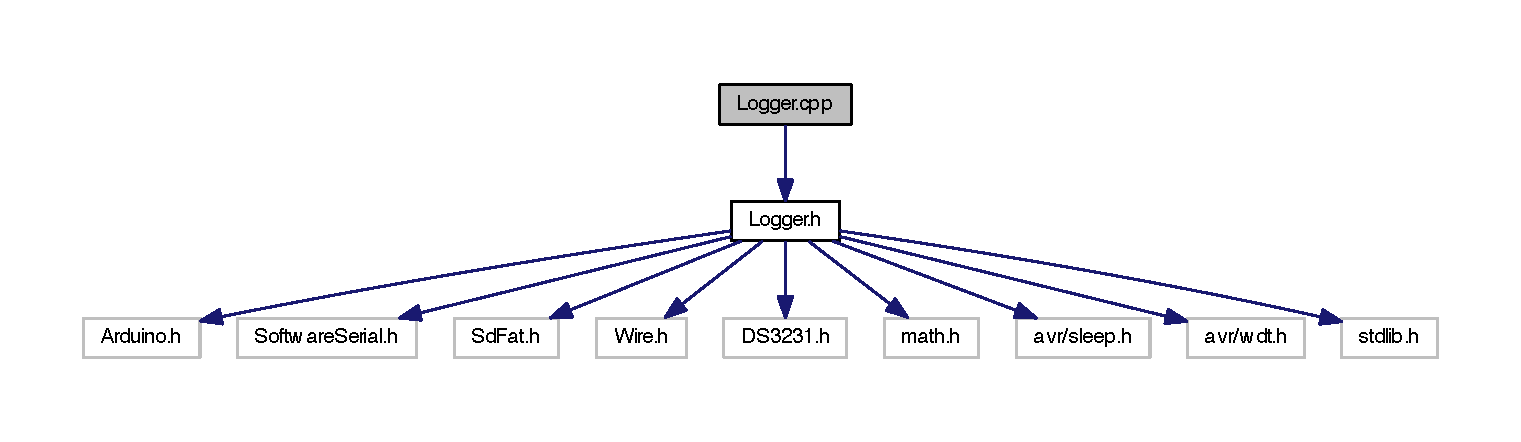
\includegraphics[width=350pt]{Logger_8cpp__incl}
\end{center}
\end{figure}
\subsection*{Macros}
\begin{DoxyCompactItemize}
\item 
\#define {\bfseries cbi}(sfr,  bit)~(\+\_\+\+S\+F\+R\+\_\+\+B\+Y\+TE(sfr) \&= $\sim$\+\_\+\+BV(bit))\hypertarget{Logger_8cpp_ae70baf5399951da1e7ad45a0ed890832}{}\label{Logger_8cpp_ae70baf5399951da1e7ad45a0ed890832}

\item 
\#define {\bfseries sbi}(sfr,  bit)~(\+\_\+\+S\+F\+R\+\_\+\+B\+Y\+TE(sfr) $\vert$= \+\_\+\+BV(bit))\hypertarget{Logger_8cpp_ac4a5536d9bf092116f88b94797ddc882}{}\label{Logger_8cpp_ac4a5536d9bf092116f88b94797ddc882}

\end{DoxyCompactItemize}
\subsection*{Functions}
\begin{DoxyCompactItemize}
\item 
void {\bfseries wake\+Up\+Now} ()\hypertarget{Logger_8cpp_adee29828901ea1b4f99ce305fa3e17bd}{}\label{Logger_8cpp_adee29828901ea1b4f99ce305fa3e17bd}

\item 
void {\bfseries wake\+Up\+Now\+\_\+tip} ()\hypertarget{Logger_8cpp_a1a3b380e75d68eef4c3913816773e1b5}{}\label{Logger_8cpp_a1a3b380e75d68eef4c3913816773e1b5}

\item 
datafile {\bfseries print} (T, 4)\hypertarget{Logger_8cpp_ad948da93eeff8ecd336bce8a4dc8736c}{}\label{Logger_8cpp_ad948da93eeff8ecd336bce8a4dc8736c}

\item 
datafile {\bfseries print} (F(\char`\"{},\char`\"{}))\hypertarget{Logger_8cpp_aa244f46a943139f91b84aac0134886b0}{}\label{Logger_8cpp_aa244f46a943139f91b84aac0134886b0}

\item 
void {\bfseries \+\_\+\+I\+S\+R\+\_\+void} ()\hypertarget{Logger_8cpp_a9c215a00c214c880d04481d256d8d522}{}\label{Logger_8cpp_a9c215a00c214c880d04481d256d8d522}

\item 
void {\bfseries \+\_\+anemometer\+\_\+count\+\_\+increment} ()\hypertarget{Logger_8cpp_aa2e4ccb5b638347db4da535aac7ac209}{}\label{Logger_8cpp_aa2e4ccb5b638347db4da535aac7ac209}

\end{DoxyCompactItemize}
\subsection*{Variables}
\begin{DoxyCompactItemize}
\item 
const int {\bfseries bottle\+\_\+logger} =0\hypertarget{Logger_8cpp_a82b81447a86ec4d16506a446ead2d959}{}\label{Logger_8cpp_a82b81447a86ec4d16506a446ead2d959}

\item 
const int {\bfseries big\+\_\+log} =1\hypertarget{Logger_8cpp_a6e587b3167201135d66e618bc4e9d6eb}{}\label{Logger_8cpp_a6e587b3167201135d66e618bc4e9d6eb}

\item 
const int {\bfseries log\+\_\+mega} =2\hypertarget{Logger_8cpp_aa77c5809820d08b6b9906e4d5cc5c282}{}\label{Logger_8cpp_aa77c5809820d08b6b9906e4d5cc5c282}

\item 
const int {\bfseries S\+C\+Kpin} = 13\hypertarget{Logger_8cpp_aac8b4ff3c3a72eabbce5302c6a62b674}{}\label{Logger_8cpp_aac8b4ff3c3a72eabbce5302c6a62b674}

\item 
const int {\bfseries M\+I\+S\+Opin} = 12\hypertarget{Logger_8cpp_a89a5801f20cfb155fbae7a349e70da2a}{}\label{Logger_8cpp_a89a5801f20cfb155fbae7a349e70da2a}

\item 
const int {\bfseries M\+O\+S\+Ipin} = 11\hypertarget{Logger_8cpp_a7e790e9a217d45f2a6d85379bef6baad}{}\label{Logger_8cpp_a7e790e9a217d45f2a6d85379bef6baad}

\item 
const int {\bfseries C\+Spin} = 10\hypertarget{Logger_8cpp_a99da311d248bcae3ed3e157271f257a2}{}\label{Logger_8cpp_a99da311d248bcae3ed3e157271f257a2}

\item 
const int {\bfseries S\+D\+Apin} = A4\hypertarget{Logger_8cpp_a3e30838b685431b8951ec64dadf77804}{}\label{Logger_8cpp_a3e30838b685431b8951ec64dadf77804}

\item 
const int {\bfseries S\+C\+Lpin} = A5\hypertarget{Logger_8cpp_ad73f03b48a5c4f2b5dc2b5baf2b8e11a}{}\label{Logger_8cpp_ad73f03b48a5c4f2b5dc2b5baf2b8e11a}

\item 
const int {\bfseries Sensor\+Power\+Pin} = 4\hypertarget{Logger_8cpp_aac01d19cf572390930779f0cccb7e32d}{}\label{Logger_8cpp_aac01d19cf572390930779f0cccb7e32d}

\item 
const int {\bfseries S\+Dpower\+Pin} = 8\hypertarget{Logger_8cpp_a273294c2c60fa9968084103809f483c3}{}\label{Logger_8cpp_a273294c2c60fa9968084103809f483c3}

\item 
const int {\bfseries Clock\+Power\+Pin} = 6\hypertarget{Logger_8cpp_a59aa6300313960491e43e02f7aa48bc4}{}\label{Logger_8cpp_a59aa6300313960491e43e02f7aa48bc4}

\item 
const int {\bfseries L\+E\+Dpin} = 9\hypertarget{Logger_8cpp_a82504a11fb254521fd47f38bc9140370}{}\label{Logger_8cpp_a82504a11fb254521fd47f38bc9140370}

\item 
const int {\bfseries wake\+Pin} = 2\hypertarget{Logger_8cpp_ad48994183e177d334acf26db183b4c02}{}\label{Logger_8cpp_ad48994183e177d334acf26db183b4c02}

\item 
const int {\bfseries interrupt\+Num} = wake\+Pin-\/2\hypertarget{Logger_8cpp_aa7fe2f17315370b6970682d6e886a39a}{}\label{Logger_8cpp_aa7fe2f17315370b6970682d6e886a39a}

\item 
const int {\bfseries manual\+Wake\+Pin} = 5\hypertarget{Logger_8cpp_a3b3aee00057d1c0000acb96c8a1ae039}{}\label{Logger_8cpp_a3b3aee00057d1c0000acb96c8a1ae039}

\item 
int {\bfseries day\+Interval}\hypertarget{Logger_8cpp_a164655a5a5c1e0540e8a7068d14ce45d}{}\label{Logger_8cpp_a164655a5a5c1e0540e8a7068d14ce45d}

\item 
int {\bfseries hour\+Interval}\hypertarget{Logger_8cpp_ab77f56a33b8532217ce48f0b1245b612}{}\label{Logger_8cpp_ab77f56a33b8532217ce48f0b1245b612}

\item 
int {\bfseries min\+Interval}\hypertarget{Logger_8cpp_a02b6432e3c27c53a8dec52bdb89e727d}{}\label{Logger_8cpp_a02b6432e3c27c53a8dec52bdb89e727d}

\item 
int {\bfseries sec\+Interval}\hypertarget{Logger_8cpp_a3f8ea935eb97b1591ba876e9b9f5696c}{}\label{Logger_8cpp_a3f8ea935eb97b1591ba876e9b9f5696c}

\item 
int {\bfseries \+\_\+days}\hypertarget{Logger_8cpp_af007ef3fe6449bc365597a159ef593c0}{}\label{Logger_8cpp_af007ef3fe6449bc365597a159ef593c0}

\item 
int {\bfseries \+\_\+hours}\hypertarget{Logger_8cpp_ae9e72989946d1faad54881543c608cd0}{}\label{Logger_8cpp_ae9e72989946d1faad54881543c608cd0}

\item 
int {\bfseries \+\_\+minutes}\hypertarget{Logger_8cpp_aa8cbf9c20655f9f019790baf6a71e073}{}\label{Logger_8cpp_aa8cbf9c20655f9f019790baf6a71e073}

\item 
int {\bfseries \+\_\+seconds}\hypertarget{Logger_8cpp_a7084691e96b1daa3a2d70def71aaf1d9}{}\label{Logger_8cpp_a7084691e96b1daa3a2d70def71aaf1d9}

\item 
bool {\bfseries \+\_\+use\+\_\+sleep\+\_\+mode} = true\hypertarget{Logger_8cpp_a68393fac7d89166dd2dcfb912a1719d3}{}\label{Logger_8cpp_a68393fac7d89166dd2dcfb912a1719d3}

\item 
bool {\bfseries C\+A\+M\+E\+R\+A\+\_\+\+I\+S\+\_\+\+ON} = false\hypertarget{Logger_8cpp_a708f1306493fcf4780f4b3fee9913ca4}{}\label{Logger_8cpp_a708f1306493fcf4780f4b3fee9913ca4}

\item 
bool {\bfseries I\+S\+\_\+\+L\+O\+G\+G\+I\+NG} = false\hypertarget{Logger_8cpp_adf875ef298ce84c624410441199174a7}{}\label{Logger_8cpp_adf875ef298ce84c624410441199174a7}

\item 
char $\ast$ {\bfseries filename}\hypertarget{Logger_8cpp_aeac90097f29f7529968697163cea5c18}{}\label{Logger_8cpp_aeac90097f29f7529968697163cea5c18}

\item 
char $\ast$ {\bfseries logger\+\_\+name}\hypertarget{Logger_8cpp_a0ac67755b34868235cbf497710a5f3c4}{}\label{Logger_8cpp_a0ac67755b34868235cbf497710a5f3c4}

\item 
bool {\bfseries ext\+Int}\hypertarget{Logger_8cpp_a8ba3a8d681fc12076bc941ab2dfe11aa}{}\label{Logger_8cpp_a8ba3a8d681fc12076bc941ab2dfe11aa}

\item 
bool {\bfseries N\+E\+W\+\_\+\+R\+A\+I\+N\+\_\+\+B\+U\+C\+K\+E\+T\+\_\+\+T\+IP} = false\hypertarget{Logger_8cpp_aac008d9b5fb23b399e3d3acfcf598355}{}\label{Logger_8cpp_aac008d9b5fb23b399e3d3acfcf598355}

\item 
bool {\bfseries L\+O\+G\+\_\+\+A\+L\+L\+\_\+\+S\+E\+N\+S\+O\+R\+S\+\_\+\+O\+N\+\_\+\+B\+U\+C\+K\+E\+T\+\_\+\+T\+IP}\hypertarget{Logger_8cpp_a3907b2190de8be0458e0ba44d05aadd5}{}\label{Logger_8cpp_a3907b2190de8be0458e0ba44d05aadd5}

\item 
unsigned int {\bfseries rotation\+\_\+count} = 0\hypertarget{Logger_8cpp_a0ece0ecf78205e2187d9bd98896e6121}{}\label{Logger_8cpp_a0ece0ecf78205e2187d9bd98896e6121}

\item 
R\+T\+Clib {\bfseries R\+TC}\hypertarget{Logger_8cpp_a65da607d8fc2158dfe99dc25bd7f0a93}{}\label{Logger_8cpp_a65da607d8fc2158dfe99dc25bd7f0a93}

\item 
D\+S3231 {\bfseries Clock}\hypertarget{Logger_8cpp_a3a6ff5c7ec928df3cd8c33fb3a263bdf}{}\label{Logger_8cpp_a3a6ff5c7ec928df3cd8c33fb3a263bdf}

\item 
Sd\+Fat {\bfseries sd}\hypertarget{Logger_8cpp_a15e6b7e1f0fb2d1e0fe1654721bb5302}{}\label{Logger_8cpp_a15e6b7e1f0fb2d1e0fe1654721bb5302}

\item 
Sd\+File {\bfseries datafile}\hypertarget{Logger_8cpp_a1115547a6eea844c4f66793a4f7d6329}{}\label{Logger_8cpp_a1115547a6eea844c4f66793a4f7d6329}

\item 
Sd\+File {\bfseries otherfile}\hypertarget{Logger_8cpp_abf344448e6a83213262a3d1b902b192f}{}\label{Logger_8cpp_abf344448e6a83213262a3d1b902b192f}

\item 
Date\+Time {\bfseries now}\hypertarget{Logger_8cpp_ac023874b2154eac7297a7575008605fe}{}\label{Logger_8cpp_ac023874b2154eac7297a7575008605fe}

\item 
float {\bfseries T0} = T0degC + 273.\+15\hypertarget{Logger_8cpp_a4211ba1269f650e21964d32238a460b2}{}\label{Logger_8cpp_a4211ba1269f650e21964d32238a460b2}

\item 
float {\bfseries Rinf} = R0$\ast$exp(-\/B/T0)\hypertarget{Logger_8cpp_a64422a8cc6d3d23d8594ae6ca4981b18}{}\label{Logger_8cpp_a64422a8cc6d3d23d8594ae6ca4981b18}

\item 
float {\bfseries T} = B / log(Rtherm/Rinf)\hypertarget{Logger_8cpp_a41cbf5427272bfe22626d2473a63f2d4}{}\label{Logger_8cpp_a41cbf5427272bfe22626d2473a63f2d4}

\end{DoxyCompactItemize}


\subsection{Detailed Description}
Data logger library Designed for the A\+Log Modules should work for any Arduino-\/based board with minimal modificiation Goals\+: (1) Manage logger utility functions, largely behind-\/the-\/scenes (2) Simplify data logger operations to one-\/line calls

Written by Andy Wickert, 2011-\/2016, and Chad Sandell, 2016 Started 27 September 2011

Designed to greatly simplify Arduino sketches for the A\+Log and reduce what the end user needs to do into relatively simple one-\/line calls.

\subsection*{L\+I\+C\+E\+N\+SE\+: G\+NU G\+PL v3}

\hyperlink{Logger_8cpp}{Logger.\+cpp} is part of \hyperlink{classLogger}{Logger}, an Arduino library written by Andrew D. Wickert and Chad T. Sandell Copyright (C) 2011-\/2015, Andrew D. Wickert Copyright (C) 2016, Andrew D. Wickert and Chad T. Sandell

This program is free software\+: you can redistribute it and/or modify it under the terms of the G\+NU General Public License as published by the Free Software Foundation, either version 3 of the License, or (at your option) any later version.

This program is distributed in the hope that it will be useful, but W\+I\+T\+H\+O\+UT A\+NY W\+A\+R\+R\+A\+N\+TY; without even the implied warranty of M\+E\+R\+C\+H\+A\+N\+T\+A\+B\+I\+L\+I\+TY or F\+I\+T\+N\+E\+SS F\+OR A P\+A\+R\+T\+I\+C\+U\+L\+AR P\+U\+R\+P\+O\+SE. See the G\+NU General Public License for more details.

You should have received a copy of the G\+NU General Public License along with this program. If not, see \href{http://www.gnu.org/licenses/}{\tt http\+://www.\+gnu.\+org/licenses/}. 
\hypertarget{Logger_8h}{}\section{Logger.\+h File Reference}
\label{Logger_8h}\index{Logger.\+h@{Logger.\+h}}
{\ttfamily \#include $<$Arduino.\+h$>$}\newline
{\ttfamily \#include $<$Sd\+Fat.\+h$>$}\newline
{\ttfamily \#include $<$Wire.\+h$>$}\newline
{\ttfamily \#include $<$D\+S3231.\+h$>$}\newline
{\ttfamily \#include $<$math.\+h$>$}\newline
{\ttfamily \#include $<$avr/sleep.\+h$>$}\newline
{\ttfamily \#include $<$avr/wdt.\+h$>$}\newline
{\ttfamily \#include $<$stdlib.\+h$>$}\newline
{\ttfamily \#include $<$E\+E\+P\+R\+O\+M.\+h$>$}\newline
{\ttfamily \#include $<$Software\+Serial.\+h$>$}\newline
{\ttfamily \#include $<$S\+F\+E\+\_\+\+B\+M\+P180.\+h$>$}\newline
Include dependency graph for Logger.\+h\+:\nopagebreak
\begin{figure}[H]
\begin{center}
\leavevmode
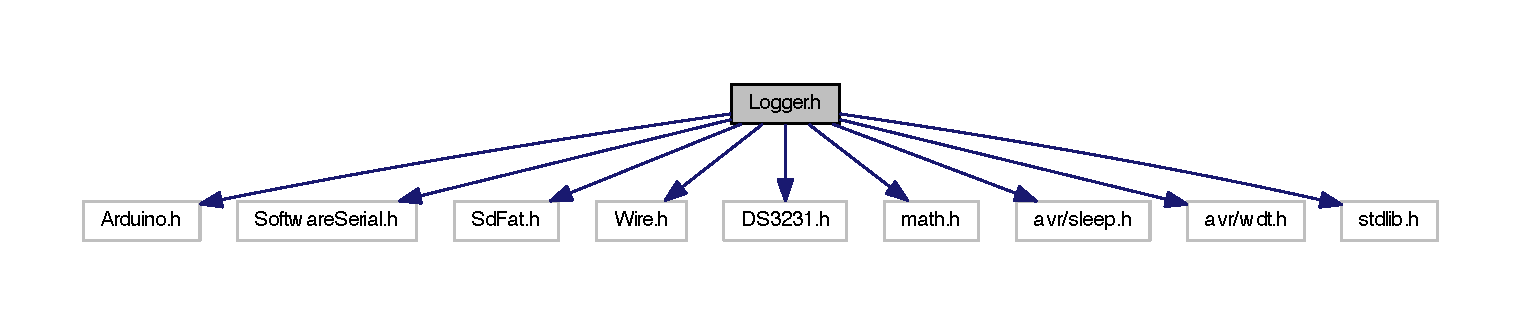
\includegraphics[width=350pt]{Logger_8h__incl}
\end{center}
\end{figure}
This graph shows which files directly or indirectly include this file\+:\nopagebreak
\begin{figure}[H]
\begin{center}
\leavevmode
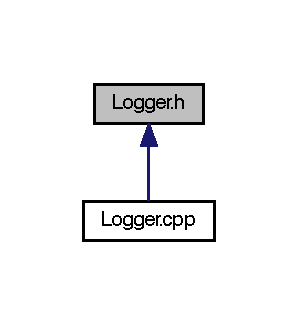
\includegraphics[width=143pt]{Logger_8h__dep__incl}
\end{center}
\end{figure}
\subsection*{Classes}
\begin{DoxyCompactItemize}
\item 
class \hyperlink{classLogger}{Logger}
\end{DoxyCompactItemize}
\subsection*{Functions}
\begin{DoxyCompactItemize}
\item 
\mbox{\Hypertarget{Logger_8h_adee29828901ea1b4f99ce305fa3e17bd}\label{Logger_8h_adee29828901ea1b4f99ce305fa3e17bd}} 
void {\bfseries wake\+Up\+Now} ()
\item 
\mbox{\Hypertarget{Logger_8h_a1a3b380e75d68eef4c3913816773e1b5}\label{Logger_8h_a1a3b380e75d68eef4c3913816773e1b5}} 
void {\bfseries wake\+Up\+Now\+\_\+tip} ()
\item 
\mbox{\Hypertarget{Logger_8h_a9c215a00c214c880d04481d256d8d522}\label{Logger_8h_a9c215a00c214c880d04481d256d8d522}} 
void {\bfseries \+\_\+\+I\+S\+R\+\_\+void} ()
\item 
\mbox{\Hypertarget{Logger_8h_aa2e4ccb5b638347db4da535aac7ac209}\label{Logger_8h_aa2e4ccb5b638347db4da535aac7ac209}} 
void {\bfseries \+\_\+anemometer\+\_\+count\+\_\+increment} ()
\item 
\mbox{\Hypertarget{Logger_8h_a7551515cf6f018df3d8d942710936aef}\label{Logger_8h_a7551515cf6f018df3d8d942710936aef}} 
void {\bfseries \+\_\+internal\+Date\+Time} (uint16\+\_\+t $\ast$date, uint16\+\_\+t $\ast$time)
\end{DoxyCompactItemize}


\subsection{Detailed Description}
\subsection*{\hyperlink{Logger_8h}{Logger.\+h}}

Data logger library header~\newline
 Designed for the A\+Log~\newline
 Modules should work for any Arduino-\/based board with minimal modificiation.~\newline
 Goals\+:
\begin{DoxyEnumerate}
\item Manage logger utility functions, largely behind-\/the-\/scenes
\item Simplify data logger operations to one-\/line calls
\end{DoxyEnumerate}

Written by Andy Wickert, 2011-\/2017, and Chad Sandell, 2017~\newline
 Started 27 September 2011

Designed to greatly simplify Arduino sketches for the A\+Log and reduce what the end user needs to do into relatively simple one-\/line calls.

\subsubsection*{L\+I\+C\+E\+N\+SE\+: G\+NU G\+PL v3}

\hyperlink{Logger_8h}{Logger.\+h} is part of \hyperlink{classLogger}{Logger}, an Arduino library written by Andrew D. Wickert and Chad T. Sandell.

Copyright (C) 2011-\/2017, Andrew D. Wickert Copyright (C) 2016-\/2017, Andrew D. Wickert and Chad T. Sandell Copyright (C) 2016-\/2017, Regents of the University of Minnesota

This program is free software\+: you can redistribute it and/or modify it under the terms of the G\+NU General Public License as published by the Free Software Foundation, either version 3 of the License, or (at your option) any later version.

This program is distributed in the hope that it will be useful, but W\+I\+T\+H\+O\+UT A\+NY W\+A\+R\+R\+A\+N\+TY; without even the implied warranty of M\+E\+R\+C\+H\+A\+N\+T\+A\+B\+I\+L\+I\+TY or F\+I\+T\+N\+E\+SS F\+OR A P\+A\+R\+T\+I\+C\+U\+L\+AR P\+U\+R\+P\+O\+SE. See the G\+NU General Public License for more details.

You should have received a copy of the G\+NU General Public License along with this program. If not, see \href{http://www.gnu.org/licenses/}{\tt http\+://www.\+gnu.\+org/licenses/}. 
%--- End generated contents ---

% Index
\backmatter
\newpage
\phantomsection
\clearemptydoublepage
\addcontentsline{toc}{chapter}{Index}
\printindex

\end{document}
